% Harus dimuat terlebih dahulu, digunakan agar file PDF memiliki format karakter yang benar.
% Untuk informasi lebih lanjut, lihat https://ctan.org/pkg/cmap.
\RequirePackage{cmap}

% Format dokumen sebagai paper konferensi menggunakan aturan IEEEtran terbaru (v1.8b).
% Untuk informasi lebih lanjut, lihat http://www.michaelshell.org/tex/ieeetran/.
\documentclass[a4paper, conference]{IEEEtran}

% Format encoding font dan input menjadi 8-bit UTF-8.
\usepackage[T1]{fontenc}
\usepackage[utf8]{inputenc}
\usepackage{amsmath}
\usepackage{enumitem}

% Digunakan untuk mengatur margin dokumen.
\usepackage{textcomp}

% Format bahasa menjadi bahasa indonesia dan inggris.
\usepackage[indonesian]{babel}

% Digunakan untuk tujuan demonstrasi.
\usepackage{mwe}

% Digunakan untuk menampilkan font dengan style yang lebih baik.
\usepackage[zerostyle=b,scaled=.75]{newtxtt}

% Digunakan untuk menampilkan tabel dengan style yang lebih baik.
\usepackage{booktabs}
\usepackage[table,xcdraw]{xcolor}
% Digunakan untuk menampilkan gambar pada dokumen.
\usepackage{graphicx}

% Digunakan untuk menampilkan potongan kode.
\usepackage{listings}
\lstset{
  basicstyle=\ttfamily,
  columns=fixed,
  basewidth=.5em,
  xleftmargin=0.5cm,
  captionpos=b
}

\usepackage{tabularx}
\usepackage{wrapfig}
% Digunakan agar backticks (`) dapat dirender pada PDF.
% Untuk informasi lebih lanjut, lihat https://tex.stackexchange.com/a/341057/9075.
\usepackage{upquote}

% Digunakan untuk menyeimbangkan bagian akhir dokumen dengan dua kolom.
\usepackage{balance}

% Kapitalisasi caption tabel
\usepackage{caption}
\captionsetup[table]{
    justification=centering, % Memusatkan caption
    labelsep=newline, % Memisahkan label "TABLE 1" dengan judul dengan baris baru
    textfont={sc}, % Membuat teks menjadi kapital
    labelfont={sc} % Membuat teks menjadi kapital
}


% Digunakan untuk menampilkan pustaka.
\usepackage[square,comma,numbers,sort&compress]{natbib}

% Mengubah format ukuran teks pada natbib.
\renewcommand{\bibfont}{\normalfont\footnotesize}

% Jika melebihi 3 penulis dapat dilakukan linebreakend 
\makeatletter
\newcommand{\linebreakand}{%
  \end{@IEEEauthorhalign}
  \hfill\mbox{}\par
  \mbox{}\hfill\begin{@IEEEauthorhalign}
}
\makeatother

% Menambah nama penulis ketika menggunakan perintah \citet.
% Untuk informasi lebih lanjut, lihat https://tex.stackexchange.com/a/76075/9075.
\usepackage{etoolbox}
\makeatletter
\patchcmd{\NAT@test}{\else \NAT@nm}{\else \NAT@hyper@{\NAT@nm}}{}{}
\makeatother

% Digunakan untuk melakukan linewrap pada pustaka dengan url yang panjang
% jika terdapat hyphens
\usepackage[hyphens]{url}

% Digunakan untuk menambah hyperlink pada referensi.
\usepackage{hyperref}

% Menonaktifkan warna dan bookmark pada hyperref.
\hypersetup{hidelinks,
  colorlinks=true,
  allcolors=black,
  pdfstartview=Fit,
  breaklinks=true
}

% Digunakan untuk membenarkan hyperref pada gambar.
\usepackage[all]{hypcap}

% Digunakan untuk menampilkan beberapa gambar
\usepackage[caption=false,font=footnotesize]{subfig}

\usepackage{stfloats}
% nama
\newcommand{\name}{Faris Rafi Pramana}
\newcommand{\authorname}{Pramana, Faris Rafi}
\newcommand{\nickname}{Faris}
\newcommand{\advisor}{Muhtadin}
\newcommand{\coadvisor}{Dion Hayu Fandiantoro}

% identitas
\newcommand{\nrp}{5024 20 1004}
\newcommand{\advisornip}{19810609 200912 1 003}
\newcommand{\coadvisornip}{1994202011064}
\newcommand{\email}{5024201004@student.its.ac.id}
\newcommand{\advisoremail}{muhtadin@te.its.ac.id}
\newcommand{\coadvisoremail}{dion@its.ac.id}

% judul
\newcommand{\tatitle}{PENGEMBANGAN SISTEM KESEIMBANGAN ROBOT
HUMANOID BERBASIS \emph{LOAD CELL}}
\newcommand{\engtatitle}{DEVELOPMENT OF A BALANCE SYSTEM FOR HUMANOID ROBOTS
BASED ON LOAD CELL}

% tempat
\newcommand{\place}{Surabaya}

% jurusan
\newcommand{\studyprogram}{Teknik Komputer}
\newcommand{\engstudyprogram}{Computer Engineering}

% fakultas
\newcommand{\faculty}{Teknologi Elektro dan Informatika Cerdas}
\newcommand{\engfaculty}{Intelligence Electrical and Informatics Technology}

% singkatan fakultas
\newcommand{\facultyshort}{FTEIC}
\newcommand{\engfacultyshort}{ELECTICS}

% departemen
\newcommand{\department}{Teknik Komputer}
\newcommand{\engdepartment}{Computer Engineering}

% Tambahkan format tanda hubung yang benar di sini
\hyphenation{
  ro-ket
  me-ngem-bang-kan
  per-hi-tu-ngan
}


\begin{document}

% Ubah kalimat berikut sesuai dengan judul penelitian.
\title{\tatitle{}}

% Ubah kalimat-kalimat berikut sesuai dengan nama, institusi, alamat dan kontak penulis.
\author{
  \IEEEauthorblockN{\name{}}
  \IEEEauthorblockA{\textit{Departemen \studyprogram{}}\\
    \textit{Institut Teknologi Sepuluh Nopember}\\
    Surabaya, Indonesia 60111\\
    \email{}}

  \and
  \IEEEauthorblockN{\advisor{}}
  \IEEEauthorblockA{\textit{Departemen \studyprogram{}}\\
    \textit{Institut Teknologi Sepuluh Nopember}\\
    Surabaya, Indonesia 60111\\
    \advisoremail{}}

  \and
  \IEEEauthorblockN{\coadvisor{}}
  \IEEEauthorblockA{\textit{Departemen \studyprogram{}}\\
    \textit{Institut Teknologi Sepuluh Nopember}\\
    Surabaya, Indonesia 60111\\
    \coadvisoremail{}}
}

% Digunakan untuk menampilkan judul dan deskripsi penulis.
\maketitle

% Mengubah keterangan `Abstract` ke bahasa indonesia.
% Hapus bagian ini untuk mengembalikan ke format awal.
\renewcommand\abstractname{Abstrak}

\begin{abstract}

  Keseimbangan dan stabilitas menjadi aspek kunci dalam pengembangan robot humanoid, terutama ketika robot harus melakukan aktivitas yang melibatkan gerakan kaki dengan tumpuan hanya pada satu kaki. Penelitian ini bertujuan untuk mengembangkan sistem keseimbangan pada robot humanoid dengan menggunakan sensor \emph{load cell} pada telapak kaki. Robot humanoid yang digunakan dalam penelitian ini menggunakan robot VI-ROSE ITS dengan total derajat kebebasan 29 DoF. Sistem ini memonitor perubahan tekanan pada kedua telapak kaki robot dan menghitung titik pusat tekanan (\textit{Center of Pressure}) terhadap robot. Perhitungan pusat teknanan tersebut menggunakan empat buah \emph{load cell} pada masing-masing telapak kaki yang diproses oleh mikrokontroler terletak pada telapak kaki dan dikirimkan ke mikrokontroler utama secara nirkabel. Kesalahan pengukuran sensor berkisar antara 0-50 gram dengan rata-rata 14.8 gram di kaki kanan dan 14.6 gram di kaki kiri. Sensor dapat mendeteksi pusat tekanan pada sumbu X dengan nilai maksimum 1.44 saat mengangkat kaki kanan dan minimum -1.33 saat mengangkat kaki kiri. Robot mampu menyeimbangkan diri menggunakan kontrol PID pada 5 servo untuk mengatur posisi \textit{roll}, dengan nilai \(K_p\) = 0.10 dan \(K_d\) = 0.005, mencapai tingkat keberhasilan 100\% dalam menjaga keseimbangan saat mengangkat kaki dengan kemiringan 3 derajat.

\end{abstract}

% Hapus bagian ini untuk mengembalikan ke format awal.
\renewcommand\IEEEkeywordsname{Kata kunci}

\begin{IEEEkeywords}

  % Ubah kata-kata berikut sesuai dengan kata kunci dari penelitian.
  Robot Humanoid, Sensor \textit{Load Cell}, Pusat Tekanan

\end{IEEEkeywords}


% Ubah bagian berikut sesuai dengan konten-konten yang akan dimasukkan pada dokumen
% Ubah judul dan label berikut sesuai dengan yang diinginkan.
\section{Pendahuluan}
\label{sec:pendahuluan}

Dalam beberapa tahun terakhir, perkembangan pesat dalam bidang robotika telah mengubah cara interaksi antara manusia dan robot, terutama dalam konteks robot humanoid\cite{chiang2020posture}. Salah satu aspek kunci dalam perancangan robot humanoid adalah menjaga keseimbangan dan stabilitas, khususnya ketika robot melakukan aktivitas yang melibatkan gerakan kaki dengan dukungan pada satu kaki. Hal ini menjadi sangat krusial dalam perlombaan robot tari, di mana robot harus mampu mempertahankan keseimbangan dan berjalan di permukaan datar dengan ketinggian yang berbeda tanpa terjatuh.

Penelitian sebelumnya telah menunjukkan berbagai pendekatan untuk mencapai keseimbangan pada robot humanoid. Misalnya, Farah Risha (2023)\cite{farah} menggunakan sensor IMU untuk memperoleh data sudut kemiringan pitch yang kemudian diproses oleh mikrokontroler untuk memperbaiki sudut pada aktuator robot. Namun, sistem ini masih belum mencapai efektivitas yang diinginkan. Di sisi lain, Arifin (2017)\cite{arifin2017implementasi} meneliti penggunaan sensor tekanan pada alas kaki sebagai bagian dari sistem kontrol keseimbangan. Kendala utama pada penelitian ini adalah ketidakefisienan pengiriman data melalui kabel, yang rentan terhadap gangguan pergerakan kaki.

Masalah utama yang dihadapi adalah robot masih cenderung jatuh saat terjadi gangguan ketika bertumpu pada satu kaki. Oleh karena itu, diperlukan peningkatan respons sistem terhadap perubahan keseimbangan. Sensor tekanan menawarkan solusi yang lebih akurat dalam mengukur perubahan pusat tekanan pada robot, memungkinkan sistem untuk merespons dengan cepat. Implementasi teknologi nirkabel berbasis sinyal radio berfrekuensi 2.4GHz diusulkan untuk meningkatkan efisiensi pengiriman data dari sensor tekanan pada telapak kaki.

Penelitian ini bertujuan untuk mengembangkan sistem keseimbangan pada robot humanoid yang memanfaatkan sensor tekanan dari load cell, dengan fokus pada peningkatan stabilitas robot saat bertumpu pada satu kaki. Batasan masalah yang ditetapkan mencakup statisnya bagian tubuh atas robot, jumlah derajat kebebasan pada bagian kaki, penggunaan mikrokontroler ESP32, dan definisi keseimbangan sebagai kemampuan robot untuk tidak terjatuh saat bergerak di permukaan yang tidak rata.
% Ubah judul dan label berikut sesuai dengan yang diinginkan.
\section{Tinjauan Pustaka}
\label{sec:tinjauanpustaka}

\begin{enumerate}[label=\Alph*.]
    \item Sensor Load Cell
    \label{subsec:sensorloadcell}

    \hspace*{1em} Sensor Load Cell adalah sensor yang digunakan untuk mengukur tekanan atau gaya yang diterapkan pada suatu objek. Sensor ini bekerja berdasarkan prinsip perubahan resistansi yang terjadi pada strain gauge yang terpasang pada sensor.

    \begin{figure}[h]
        \centering
        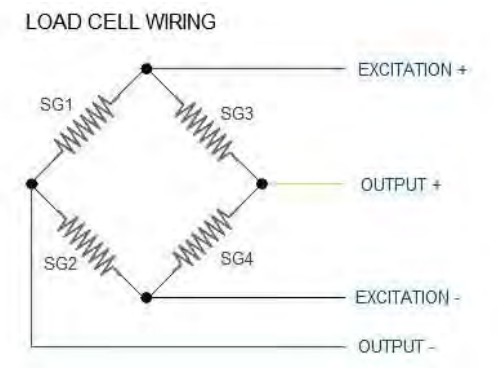
\includegraphics[width=0.3\textwidth]{./gambar/wheatstone_loadcell.png}
        \caption{Rangkaian Wheatstone Bridge pada Load Cell\cite{rahman2018autonomous}.}
        \label{fig:Wheatstone_Bridge}
    \end{figure}
    
    \begin{equation}
      V_{\mathrm{out}} = V_{\mathrm{in}} \cdot \frac{R_2 \cdot R_3 - R_1 \cdot R_4}{(R_1 + R_2) \cdot (R_3 + R_4)}
      \label{eq:Wheatstone_Bridge}
    \end{equation}
    
    \hspace*{1em} Di dalam sensor Load Cell, sistem sudah dilengkapi dengan rangkaian Wheatstone Bridge. Rangkaian Wheatstone, seperti ditunjukkan pada Gambar \ref{fig:Wheatstone_Bridge}, adalah rangkaian yang digunakan untuk mengukur perubahan resistansi yang memiliki sensitivitas tinggi \cite{rahman2018autonomous}. Untuk mengukur perubahan resistansi, digunakan persamaan Wheatstone Bridge seperti pada Persamaan \ref{eq:Wheatstone_Bridge}. 

    \item \textit{Real Time Operating System} (RTOS)
    \label{subsec:rtos}

    \hspace*{1em} Real-Time Operating System (RTOS) adalah komponen penting dalam sistem tertanam modern. Kemampuannya dalam mengelola tugas konkuren secara efektif memungkinkan sistem untuk memproses data dari berbagai sensor, seperti \emph{load cell}, secara simultan, dan mengendalikan aktuator dengan presisi tinggi \cite{sayyad2023real}. Penjadwalan tugas yang tepat waktu dan penanganan interupsi yang efisien memastikan respons cepat dan stabil dari robot, yang sangat penting dalam aplikasi robotika yang dinamis dan kompleks.

    \begin{figure} [h] \centering
      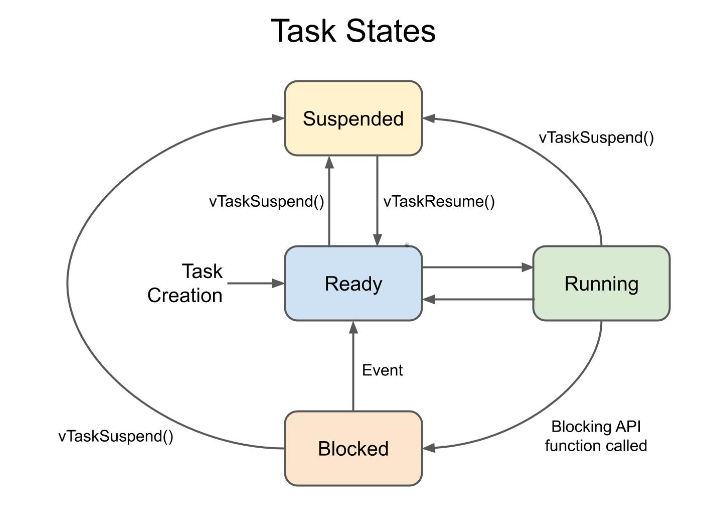
\includegraphics[scale=0.4]{gambar/rtos.png}
      \caption{Task Scheduling (RTOS)\cite{digikey2021task}.}
      \label{fig:RTOS}
    \end{figure}
  
    \hspace*{1em} State diagram pada Gambar \ref{fig:RTOS} menggambarkan bagaimana RTOS memungkinkan sistem untuk menjalankan berbagai tugas secara bersamaan, dengan memprioritaskan tugas-tugas yang lebih penting\cite{digikey2021task}. Hal ini memungkinkan robot untuk merespons dengan cepat terhadap perubahan lingkungan, seperti menjaga keseimbangan, dan secara keseluruhan meningkatkan kinerja dan adaptabilitas sistem robotika.

    \item Sistem Kontrol PID
    \label{subsec:sistemkontrolpid}

    \hspace*{1em} Penggunaan sistem kontrol PID (Proportional-Integral-Derivative) adalah metode yang umum digunakan dalam kontrol servo motor. Sistem ini membantu menjaga keseimbangan dan stabilitas robot dengan mengoreksi pergerakan berdasarkan nilai error yang dihasilkan dari perbedaan antara posisi aktual dan posisi yang diinginkan. PID terdiri dari tiga komponen utama: kontrol proporsional (P), integral (I), dan diferensial (D). Masing-masing komponen ini berfungsi untuk memperbaiki kesalahan dengan cara yang berbeda.

    \begin{equation}
      \mathrm{Koreksi} = K_p \cdot \mathrm{error} + K_i \cdot \int_{0}^{t} \mathrm{error} \cdot dt + K_d \cdot \frac{d\mathrm{error}}{dt}
    \end{equation}

    \hspace*{1em} Gabungan dari ketiga komponen ini membentuk kontrol PID yang efektif dalam menjaga keseimbangan dan stabilitas robot. Pengaturan parameter $K_p$, $K_i$, dan $K_d$ yang tepat sangat penting untuk memastikan sistem berkinerja optimal dan responsif.

    \item Pusat Tekanan
    \label{subsec:pusattekanan}

    \hspace*{1em} Pusat tekanan adalah titik dimana semua gaya terkonsentrasi pada titik tersebut tanpa ada momen torsi\cite{hawley2016external}. Dalam pusat tekanan ini terdiri dari beberapa tekanan yang kemudian dihitung nilainya berdasarkan luas penampang tersebut hingga didapatkan posisi pusat tekanan tersebut. Pusat Tekanan memiliki hubungan dengan keseimbangan robot terutama pada titik pusat gravitasi\cite{arifin2017implementasi}.

    \begin{equation}
      X_{\mathrm{cop}} = X_0 + \frac{(F2 + F4) \cdot dx}{F1 + F2 + F3 + F4}
      \label{eq:COP_X_1}
    \end{equation}

    \begin{equation}
      Y_{\mathrm{cop}} = Y_0 + \frac{(F1 + F2) \cdot dy}{F1 + F2 + F3 + F4}
      \label{eq:COP_Y_1}
    \end{equation}


    \begin{figure} [h] \centering
      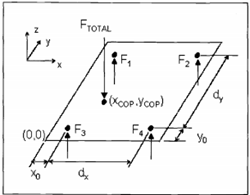
\includegraphics[width=0.3\textwidth]{gambar/Konsep_Letak.png}
      \caption{Konsep Tata Letak Pusat Tekanan\cite{resna2005}.}
      \label{fig:Konsep_Letak}
    \end{figure}

    \hspace*{1em} Gambar \ref{fig:Konsep_Letak} menunjukkan konsep peletakkan sensor tekanan. Dari konsep tersebut dapat dihitung pusat tekanan dengan menggunakanan Persamaan \ref{eq:COP_X_1} dan Persamaan \ref{eq:COP_Y_1}.
\end{enumerate}
% Ubah judul dan label berikut sesuai dengan yang diinginkan.
\section{Desain dan Implementasi}
\label{sec:desaindanimplementasi}

\begin{enumerate}[label=\Alph*.]
    \item Diagram Blok Sistem
    \label{subsec:diagrambloksistem}

    \hspace*{1em} Sistem yang telah dirancang memiliki beberapa komponen utama, yaitu bagian sensor, bagian kontrol, bagian sistem mekanik, dan bagian \textit{motion data}. 

    \begin{figure} [h] \centering
        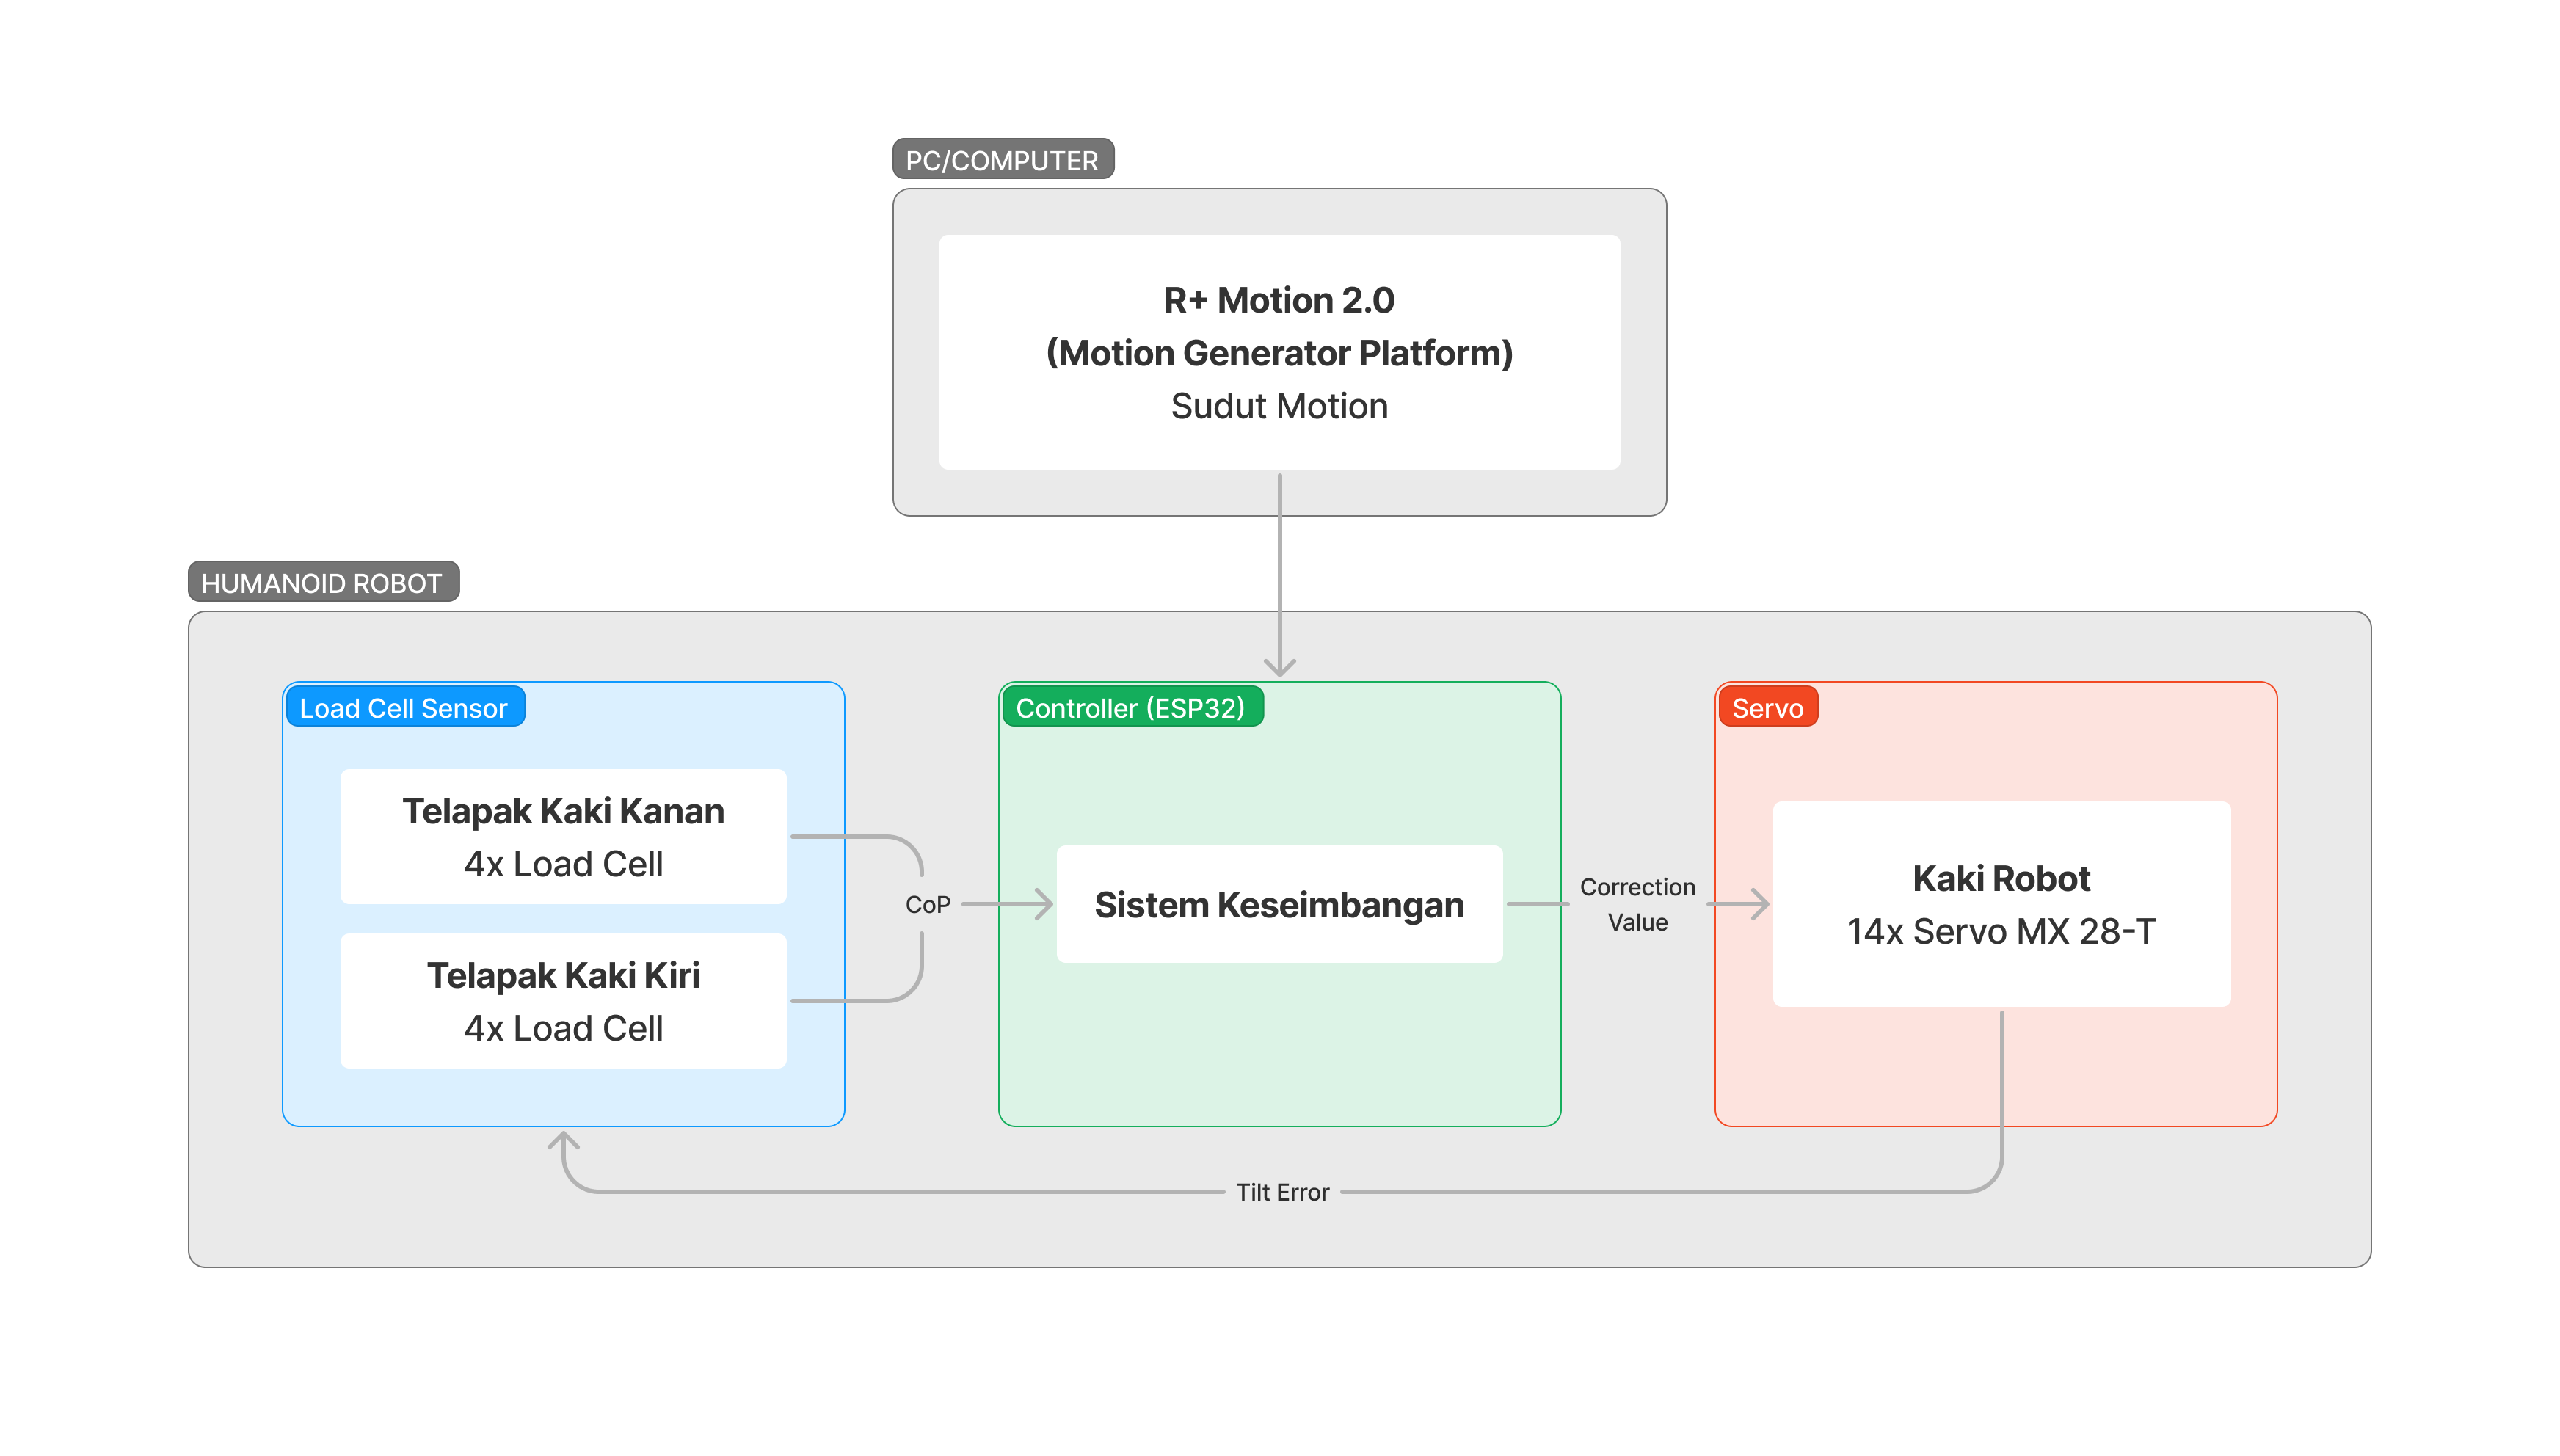
\includegraphics[width=0.45\textwidth]{gambar/Diagram_Sistem.png}
        \caption{Diagram Sistem Secara Keseluruhan}
        \label{fig:Diagram_Sistem}
    \end{figure}
    
    \hspace*{1em} Bagian sensor mencakup \emph{load cell} yang dipasang pada setiap telapak kaki robot. \emph{Load cell} ini berfungsi untuk mendeteksi beban atau tekanan pada kaki robot. Bagian kontrol melibatkan mikrokontroler yang bertanggung jawab untuk mengolah data dari sensor dan mengontrol gerakan robot. Bagian sistem mekanik mencakup kerangka robot yang terdiri dari berbagai servo yang digunakan untuk menggerakkan robot. Bagian \textit{motion data} menyimpan gerakan yang telah dirancang sebelumnya dalam sistem file mikrokontroler. Data ini terdiri dari beberapa frame yang berisi array target posisi untuk setiap servo beserta waktu yang diperlukan untuk mencapai posisi tersebut. Diagram sistem dapat dilihat pada Gambar \ref{fig:Diagram_Sistem}.
    
    \item Sistem Mekanik
    \label{subsec:sistemmekanik}

    \hspace*{1em} Desain tubuh robot humanoid ini mencakup 29 derajat kebebasan. Tubuh bagian atas menggunakan 15 servo tipe XL-320, sedangkan tubuh bagian bawah menggunakan 14 servo tipe MX-28. Rincian desain, ukuran, dan penamaan ID servo pada robot dapat dilihat pada Gambar \ref{fig:Desain_Mekanik}. 

    \begin{figure} [h] \centering
      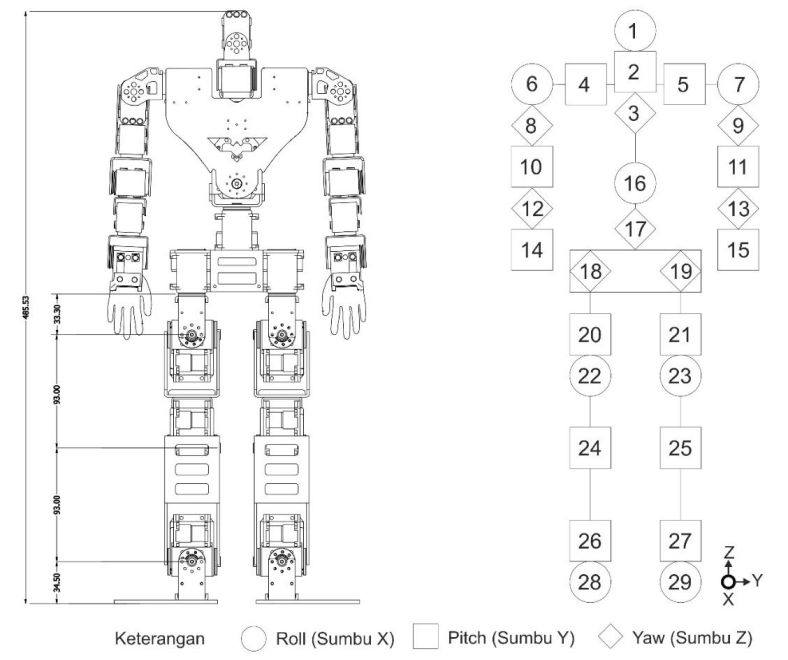
\includegraphics[width=0.35\textwidth]{gambar/Desain_Mekanik.png}
      \caption{Desain Mekanik Robot dan Penamaan ID Servo}
      \label{fig:Desain_Mekanik}
    \end{figure}

    \item Sistem Elektronik
    \label{subsec:sistemelektronik}

    \hspace*{1em} Sistem perangkat keras (hardware) dalam penelitian ini dijelaskan melalui diagram blok yang ditunjukkan pada Gambar \ref{fig:Diagram_Elektronik}. Sistem ini menggunakan sistem tertanam yang terdiri dari mikrokontroler ESP32 dan ESP32-C3. Sistem tertanam dipilih karena robot yang dikembangkan dalam penelitian ini merupakan pengembangan dari penelitian sebelumnya yang dilakukan oleh Fahd (2018)\cite{fahd}. 

    \begin{figure} [h] \centering
      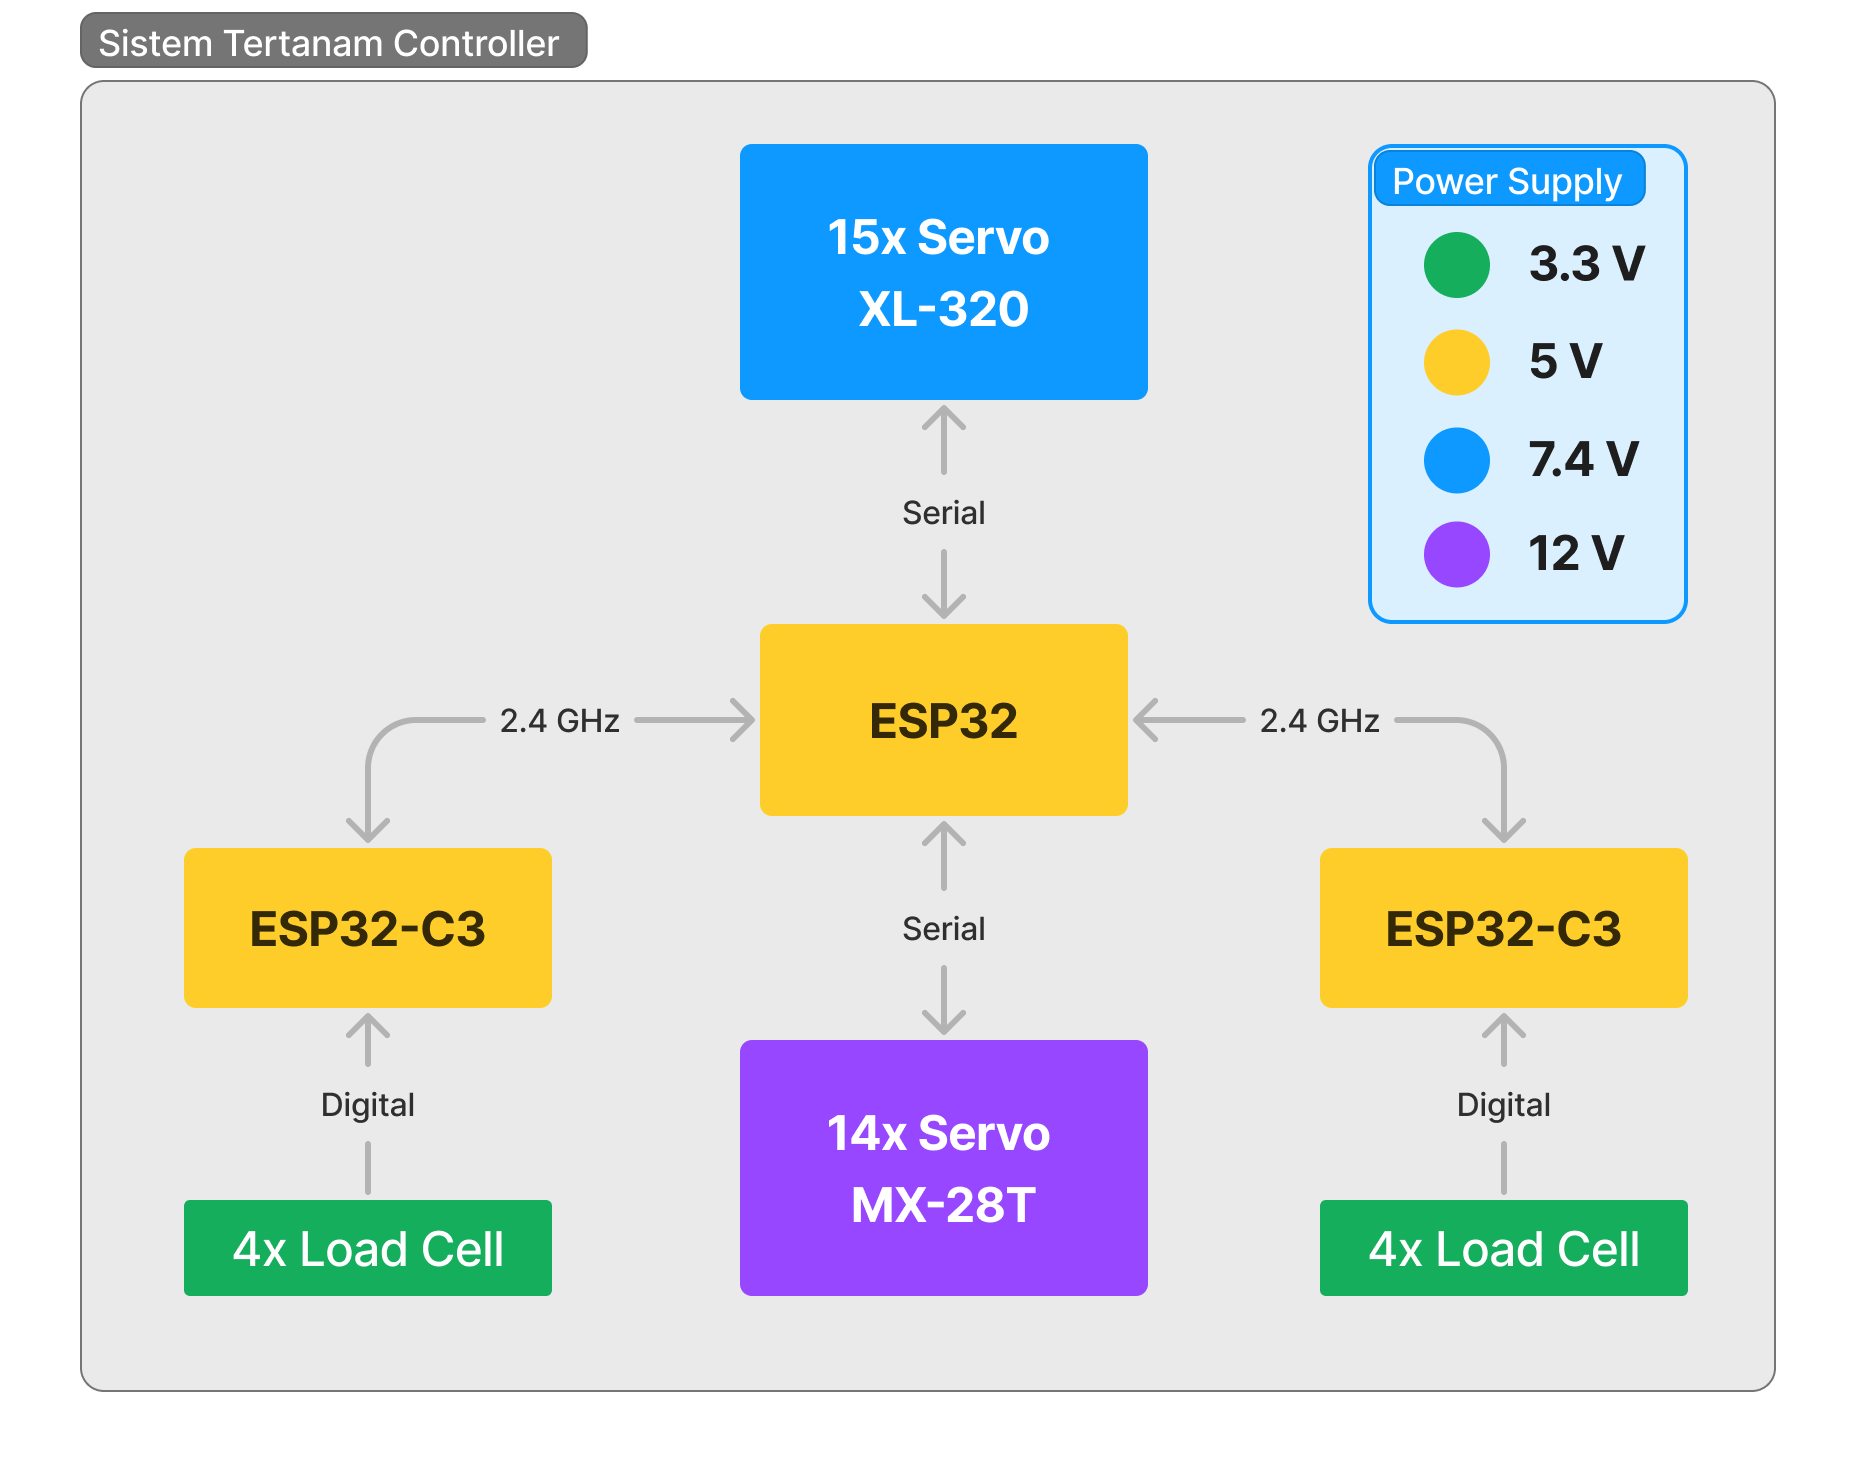
\includegraphics[width=0.4\textwidth]{gambar/Diagram_Elektronik.png}
      \caption{Diagram Elektronik dan Komunikasi Antar Komponen}
      \label{fig:Diagram_Elektronik}
    \end{figure}

    \hspace*{1em} ESP32-C3, digunakan untuk pengambilan data dari load cell dan mengirimkannya ke ESP32. ESP32-C3 memiliki kemampuan Wi-Fi yang sama dengan ESP32, sehingga memungkinkan komunikasi nirkabel antara dua mikrokontroler. ESP32-C3 juga memiliki dimensi yang lebih kecil, sehingga lebih mudah ditempatkan pada kaki robot.

    \item Desain Telapak Kaki Robot
    \label{subsec:desainsistemloadcell}

    \hspace*{1em} Setiap telapak kaki robot dilengkapi dengan 4 \emph{load cell} yang terpasang di ujung-ujung kaki. Masing-masing \emph{load cell} mendeteksi tekanan, sehingga memungkinkan sistem untuk menentukan posisi pusat tekanan pada telapak kaki robot. Desain telapak kaki robot dapat dilihat pada Gambar \ref{fig:Desain_Kaki}.
    
    \begin{figure} [h] \centering
      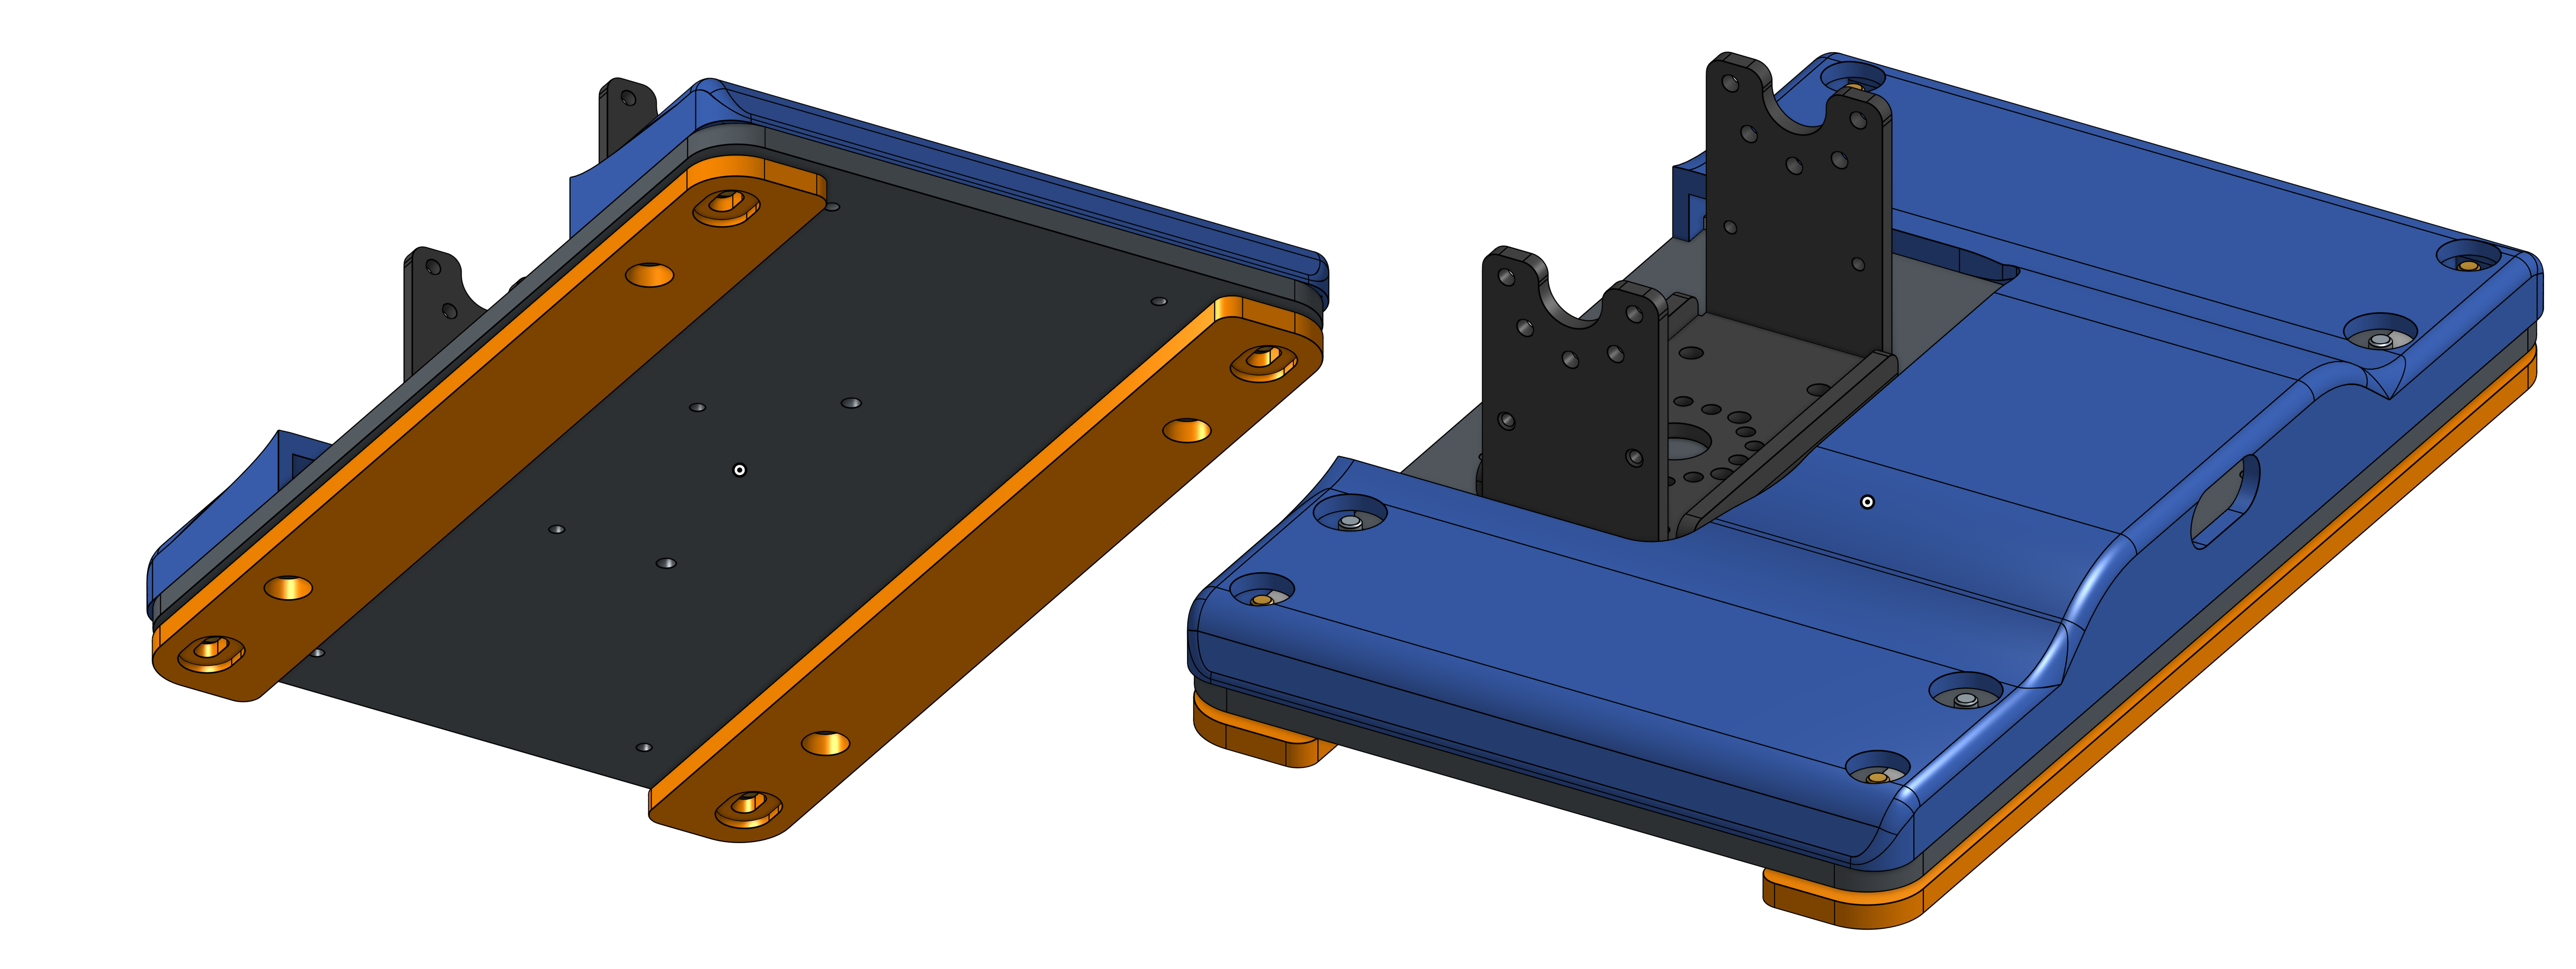
\includegraphics[width=0.4\textwidth]{gambar/Desain_Kaki.png}
      \caption{Desain Telapak Kaki Robot secara Keseluruhan}
      \label{fig:Desain_Kaki}
    \end{figure}

    \hspace*{1em} Pada Gambar \ref{fig:Desain_Kaki}, terlihat bahwa setiap \emph{load cell} ditempatkan pada ujung kaki robot. \emph{Load cell} tersebut terhubung ke mikrokontroler yang terletak di dalam kaki robot. Pada bagian elektronik, telah diberikan penutup berupa \textit{closure} yang terbuat dari 3D print untuk melindungi komponen dari kerusakan. Pada bagian mekanis, sensor \emph{load cell} dilengkapi dengan \textit{pad} yang berfungsi sebagai penekan sensor \emph{load cell} ke permukaan dan juga anti slip agar tidak mudah tergelincir.  

    \item Kongurasi Koefisien \emph{Load Cell}
    \label{subsec:konfigurasikoefisien}

    \hspace*{1em} Sebelum \emph{load cell} dapat digunakan, perlu dilakukan kalibrasi untuk mengukur koefisien \emph{load cell} dengan mengatur parameter seperti nilai koefisien \textit{scaling} dan \textit{offset}. Untuk mempermudah pengaturan, dibuatkan aplikasi konfigurasi dengan antarmuka pengguna grafis (GUI) yang mudah digunakan dan dapat diakses melalui browser. GUI ini memiliki control menu untuk mengakses fungsi dan pengaturan, serta menampilkan titik pusat tekanan yang memberikan visualisasi dampak perubahan parameter terhadap sistem. Gambar \ref{fig:Preview_Aplikasi} menunjukkan tampilan aplikasi konfigurasi, termasuk control menu dan tampilan titik pusat tekanan. Aplikasi ini akan menyimpan data konfigurasi ke dalam memori EEPROM mikrokontroler, sehingga data tetap tersimpan meskipun mikrokontroler dimatikan.

    \begin{figure} [h] \centering
      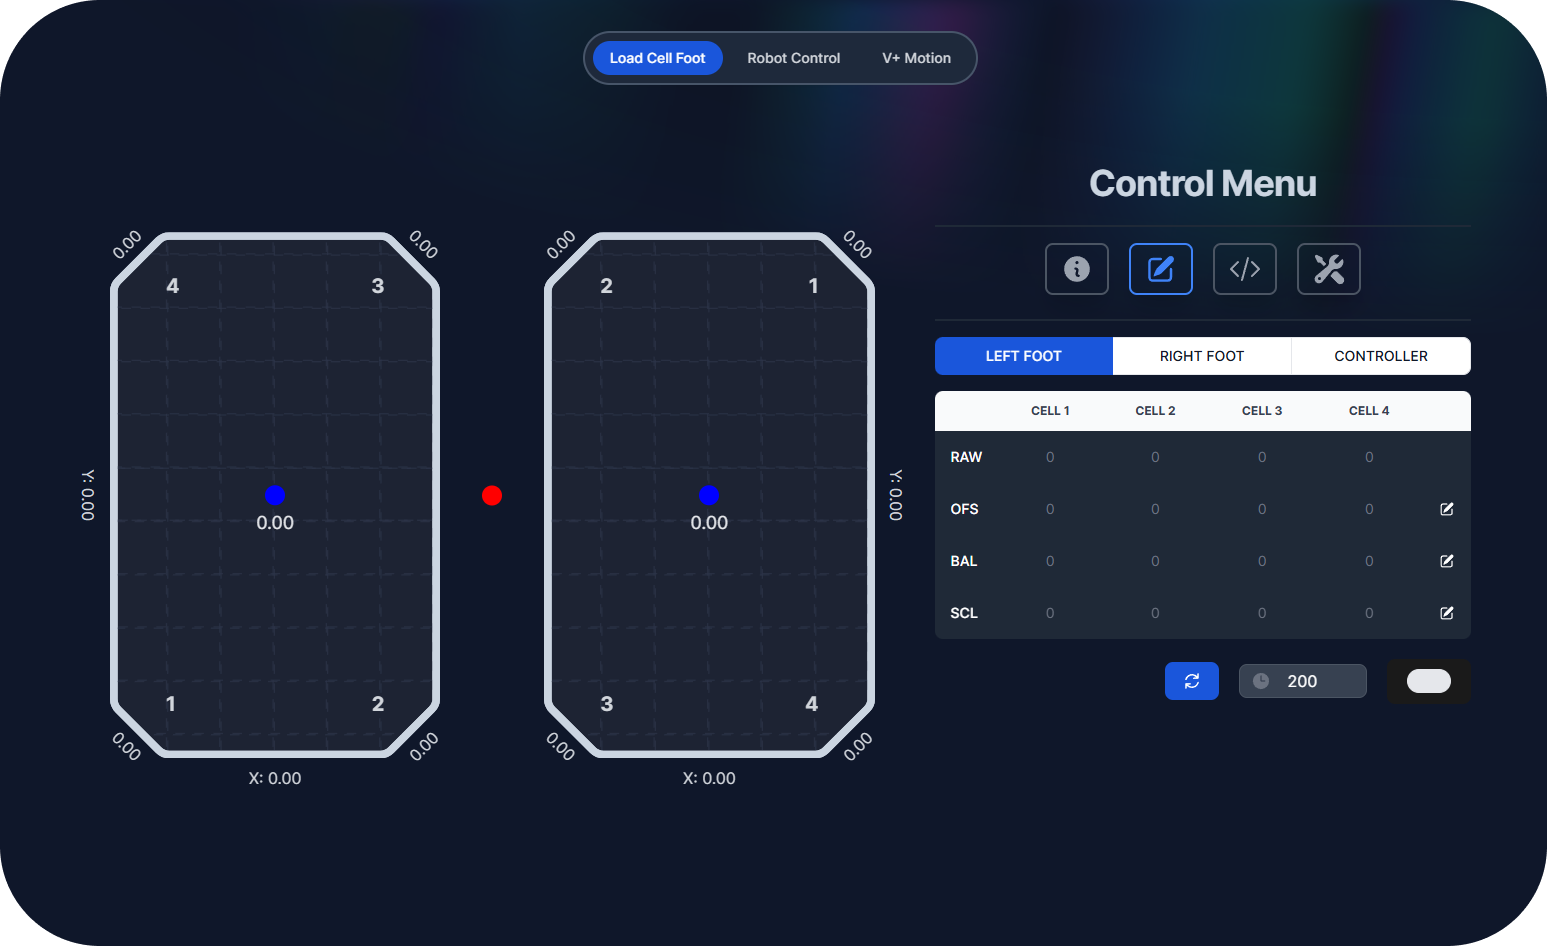
\includegraphics[width=0.4\textwidth]{gambar/preview_aplikasi.png}
      \caption{Aplikasi yang Digunakan untuk Konfigurasi \emph{Load Cell}}
      \label{fig:Preview_Aplikasi}
    \end{figure}

    \item Perhitungan Pusat Tekanan terhadap Robot
    \label{subsec:perhitunganpusattekanan}

    \hspace*{1em} Pusat tekanan pada robot dihitung dengan menggabungkan data dari kedua kaki robot. Mikrokontroler utama akan berkomunikasi dengan mikrokontroler pada kaki kiri dan kaki kanan untuk mendapatkan data pusat tekanan dan total tekanan. Data tersebut kemudian digunakan untuk mendapatkan posisi pusat tekanan terhadap robot. Perhitungan posisi pusat tekanan pada robot dilakukan seperti pada persamaan \ref{eq:Total_Force_Robot}, \ref{eq:COP_X_Robot}, dan \ref{eq:COP_Y_Robot}. 
    
    \begin{figure} [h] \centering
      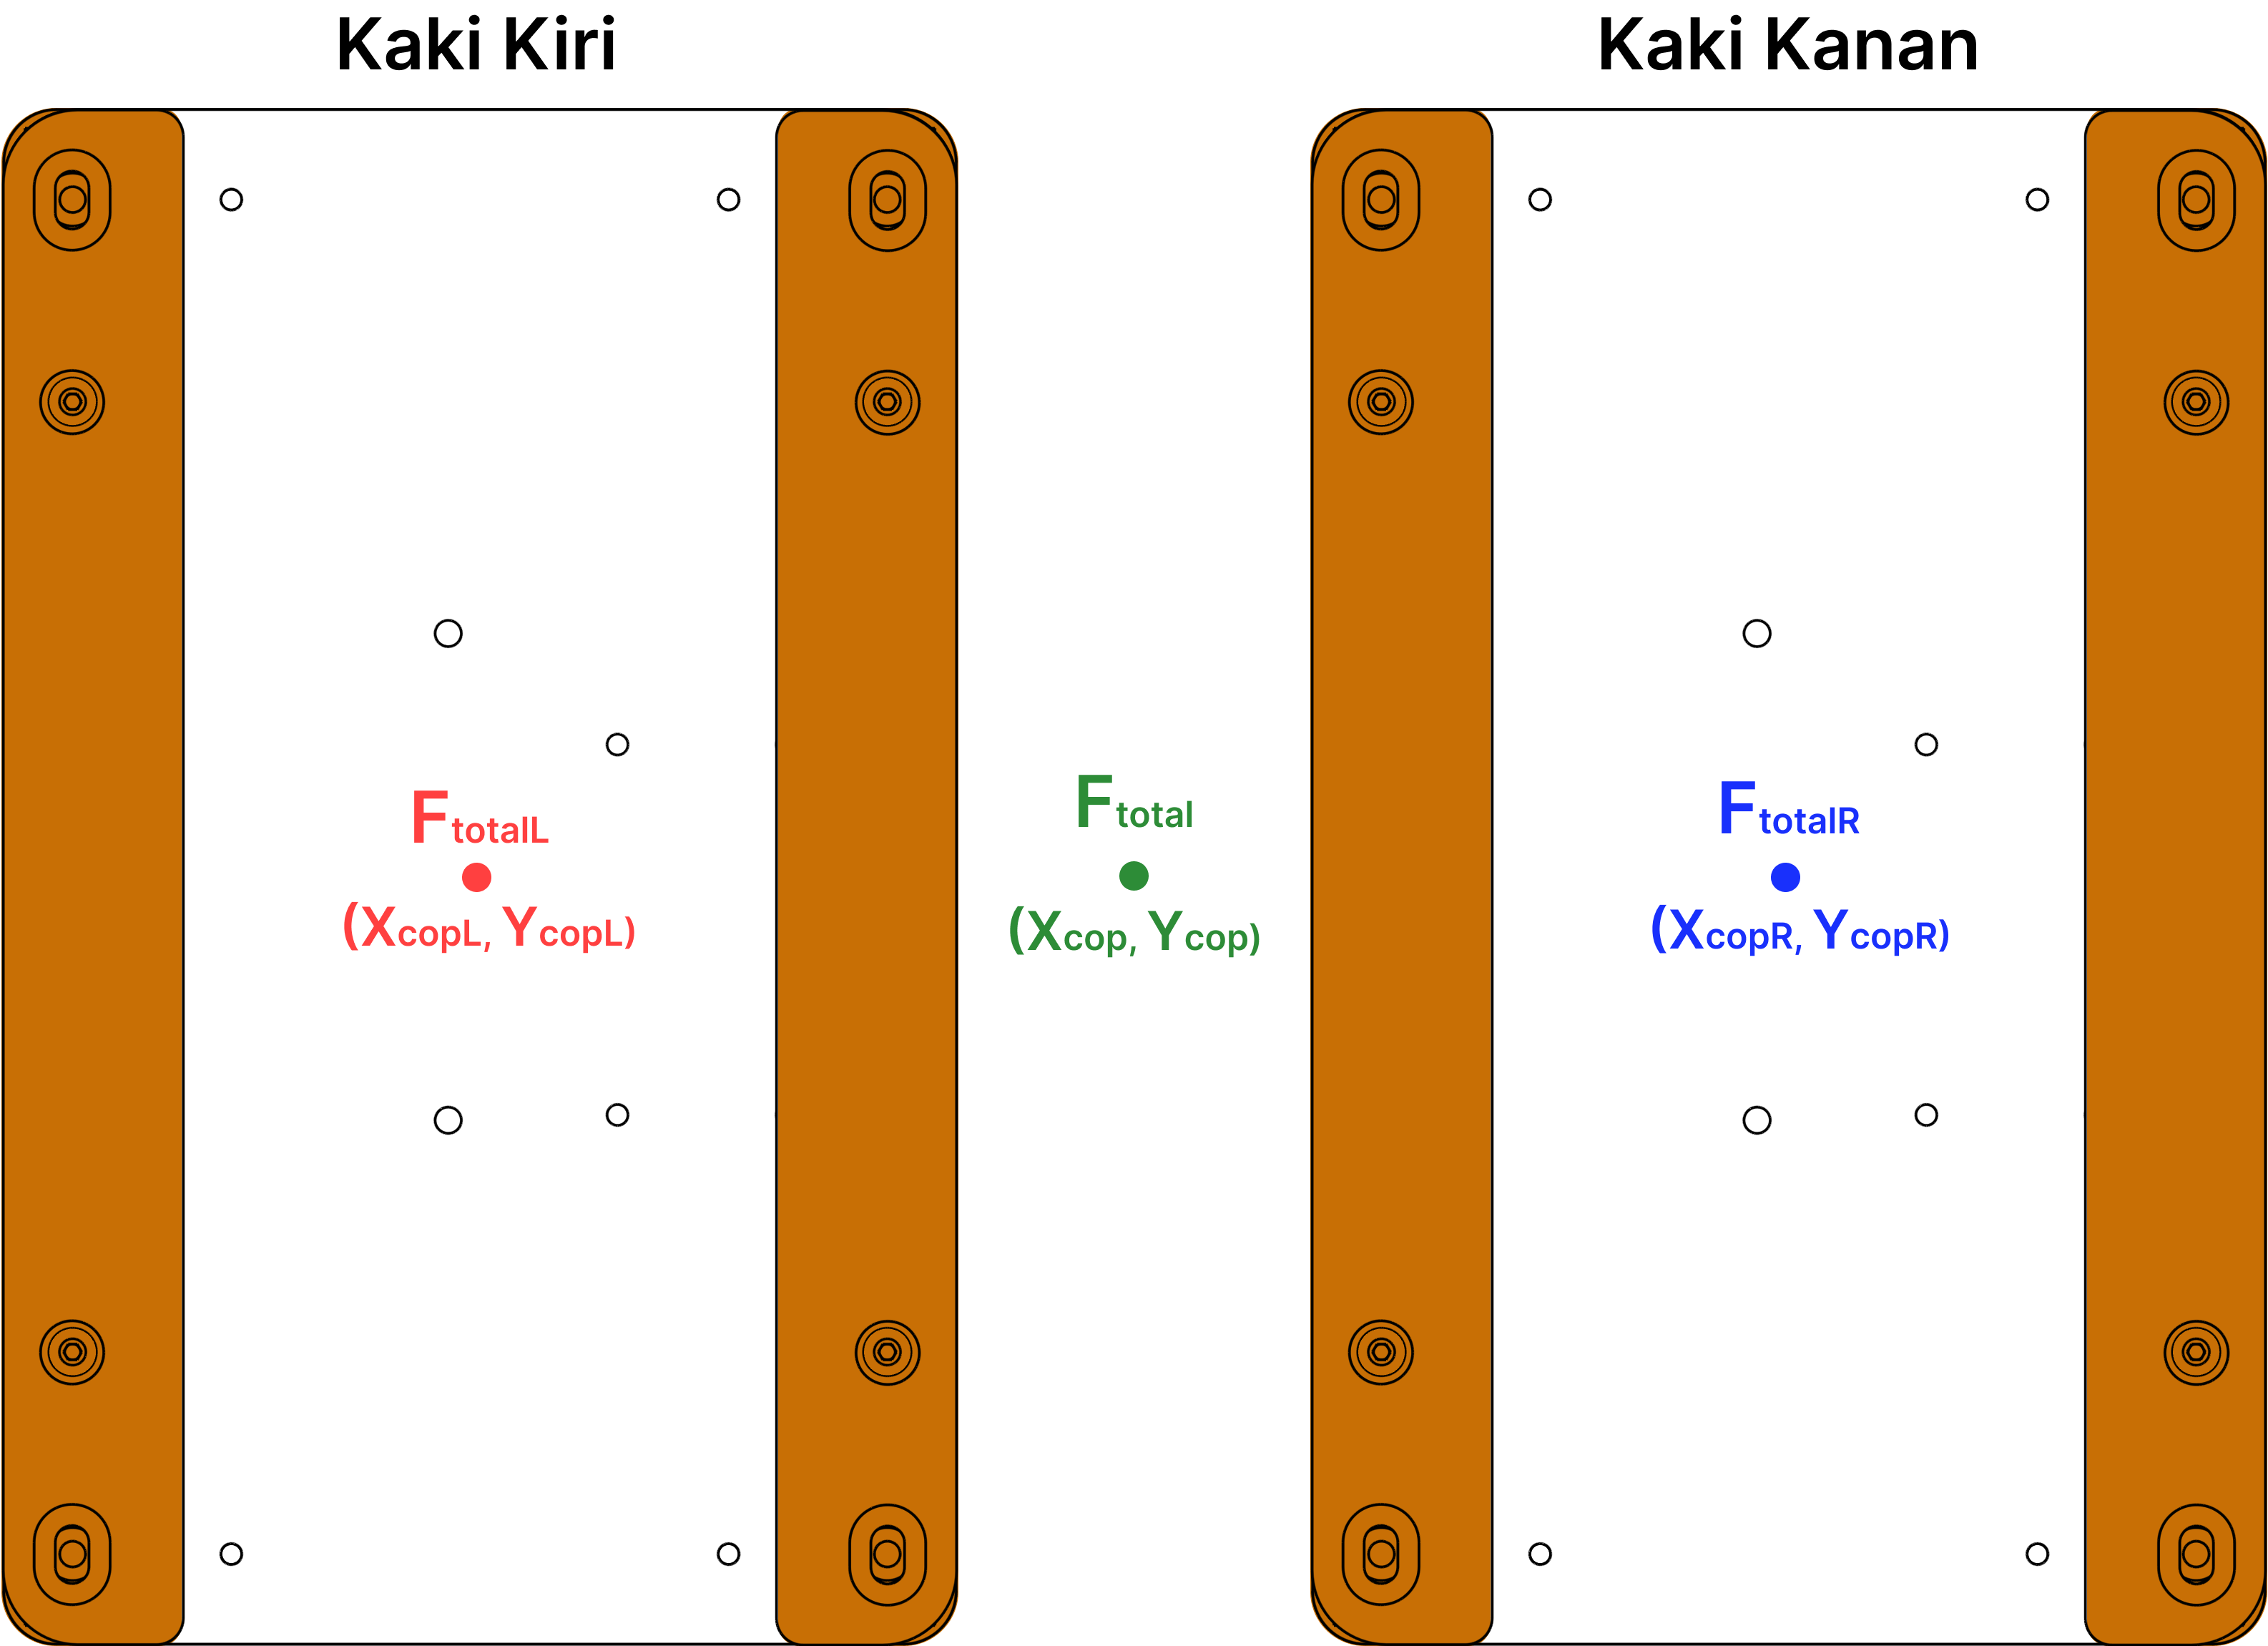
\includegraphics[width=0.4\textwidth]{gambar/COP_Robot.png}
      \caption{Pusat Tekanan pada Robot (Hijau), Pusat Tekanan pada Kaki Kiri (Merah), dan Pusat Tekanan pada Kaki Kanan (Biru)}
      \label{fig:COP_Robot}
    \end{figure}

    \begin{equation}
      F_{\mathrm{total}} = F_{\mathrm{totalL}} + F_{\mathrm{totalR}}
      \label{eq:Total_Force_Robot}
    \end{equation}

    \begin{equation}
      X_{\mathrm{cop}} = \frac{F_{\mathrm{totalL}} \cdot X_{\mathrm{copL}} + F_{\mathrm{totalR}} \cdot X_{\mathrm{copR}}}{F_{\mathrm{total}}}
      \label{eq:COP_X_Robot}
    \end{equation}

    \begin{equation}
      Y_{\mathrm{cop}} = \frac{F_{\mathrm{totalL}} \cdot Y_{\mathrm{copL}} + F_{\mathrm{totalR}} \cdot Y_{\mathrm{copR}}}{F_{\mathrm{total}}}
      \label{eq:COP_Y_Robot}
    \end{equation}

    \hspace*{1em} Data pusat tekanan pada penelitian ini akan menggunakan skala. Sesuai dengan Gambar \ref{fig:COP_Robot}, sumbu Y memiliki skala dari -1 hingga 1. Batas atas diwakili oleh nilai 1, sedangkan batas bawah diwakili oleh nilai -1. Sedangkan pada sumbu X memiliki skala dari -2 hingga 2, dengan batas kanan diwakili oleh nilai 2 dan batas kiri diwakili oleh nilai -2. Untuk sumbu X, ketika berat robot bertumpu pada salah satu kaki, nilai pusat tekanan akan bernilai positif atau negatif tergantung pada posisi kaki yang bertumpu. Ketika robot diangkat, nilai pusat tekanan akan berada pada titik (0,0) yang berada di tengah-tengah telapak kaki. 

    \item Algoritma Sistem Kontrol PID
    \label{subsec:algoritmakontrolpid}

    \hspace*{1em} Pada penelitian ini, terdapat dua kontrol PID, yaitu kontrol PID Pitch dan kontrol PID Roll. Pada kontrol PID Pitch, input berupa nilai posisi pusat tekanan pada sumbu Y. Sedangkan pada kontrol PID Roll, input berupa nilai posisi pusat tekanan pada sumbu X. Untuk setpoint kontrol PID Pitch dan Roll, digunakan nilai yang sudah ditemukan pada pengambilan data pusat tekanan sebelumnya. Pada Persamaan \ref{eq:Error_PID}, nilai error diperoleh dari selisih antara posisi pusat tekanan saat ini dengan setpoint. Kemudian, pada persamaan \ref{eq:Koreksi_PID}, nilai error digunakan untuk menghitung nilai koreksi yang akan digunakan untuk mengatur posisi servo sebagai kompensasi.

    \begin{equation}
      \mathrm{e} = COP_{\mathrm{error}} = COP_{\mathrm{set}} - COP_{\mathrm{input}}
      \label{eq:Error_PID}
    \end{equation}

    \begin{equation}
      \theta_\mathrm{e} = \mathrm{Kp} \cdot \mathrm{e} + \mathrm{Ki} \cdot \int \mathrm{e} + \mathrm{Kd} \cdot \frac{\mathrm{de}}{\mathrm{dt}}
      \label{eq:Koreksi_PID}
    \end{equation}

    \begin{figure} [h] \centering
      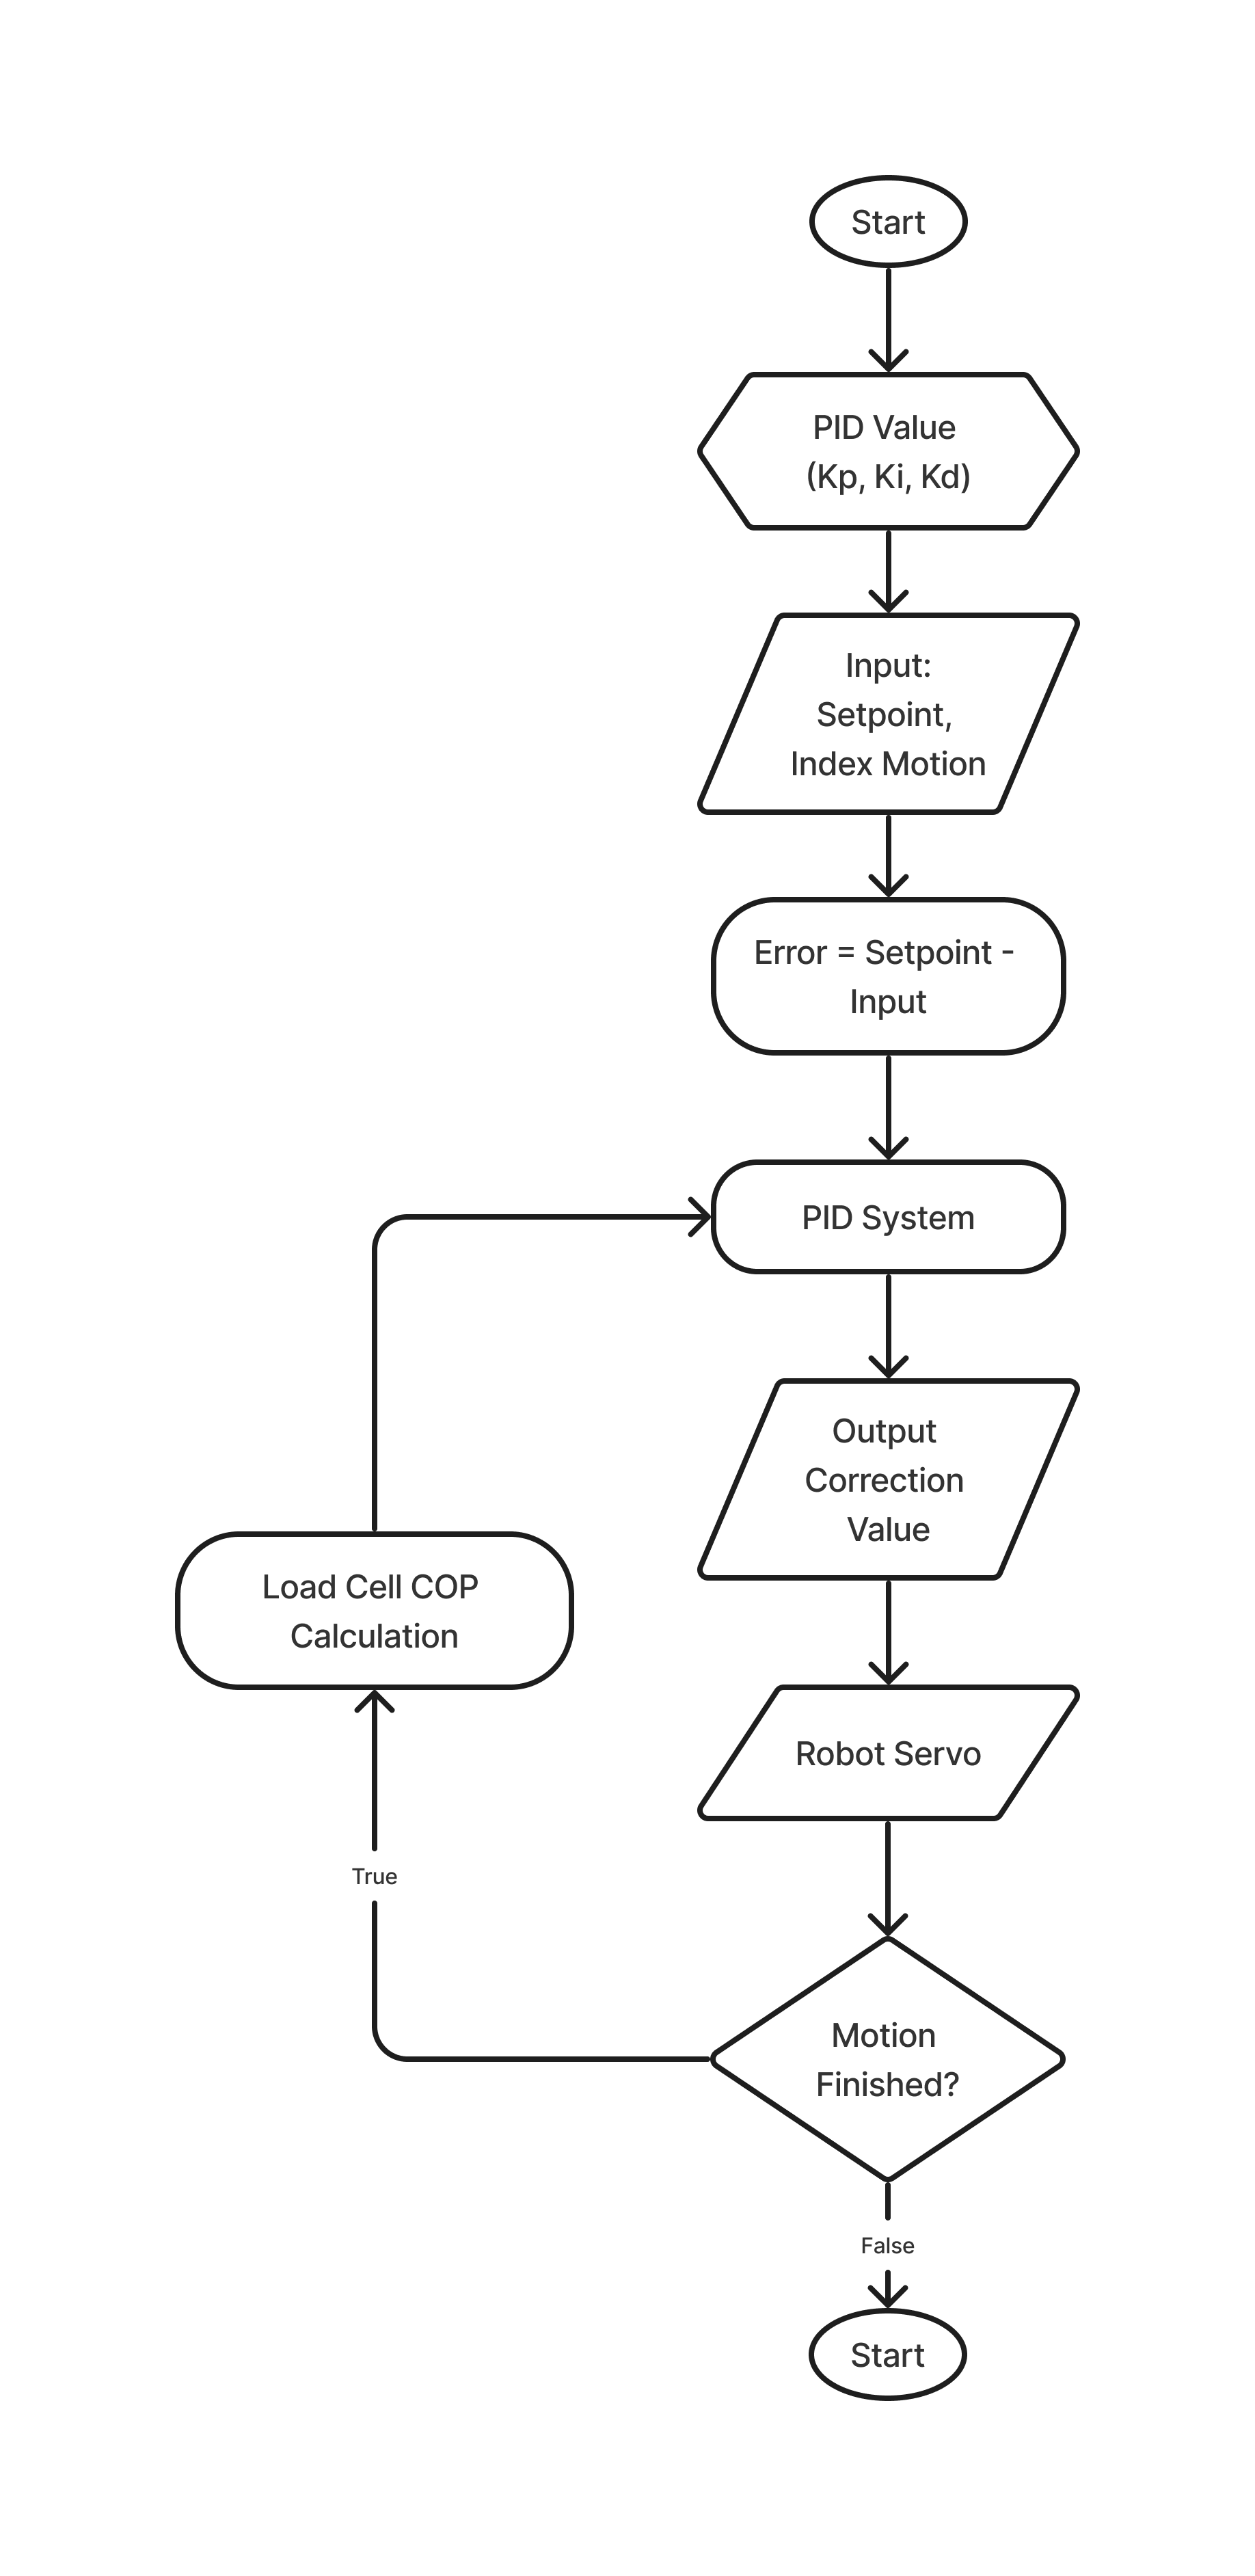
\includegraphics[width=0.38\textwidth]{gambar/Flow_Kontrol.png}
      \caption{Diagram Alir Sistem Kontrol PID Ketika \textit{Motion} Robot Berjalan}
      \label{fig:Flow_Kontrol}
    \end{figure}
    
    \hspace*{1em} Pada flowchart Gambar \ref{fig:Flow_Kontrol}, ditunjukkan tahapan respon sistem terhadap \textit{error} yang disebabkan oleh perbedaan antara posisi pusat tekanan yang diinginkan dan yang sebenarnya. Pertama, nilai PID diatur sesuai karakteristik sistem, kemudian setpoint diatur sesuai posisi pusat tekanan yang diinginkan. \textit{Error} dihitung dengan persamaan \ref{eq:Error_PID}. Nilai \textit{error} ini digunakan untuk menghitung koreksi menggunakan persamaan \ref{eq:Koreksi_PID}. Robot akan melakukan gerakan untuk menjaga keseimbangan berdasarkan koreksi yang dihasilkan oleh kontrol PID, yang berjalan terus menerus hingga \textit{motion} robot selesai.

    \begin{figure} [h] \centering
      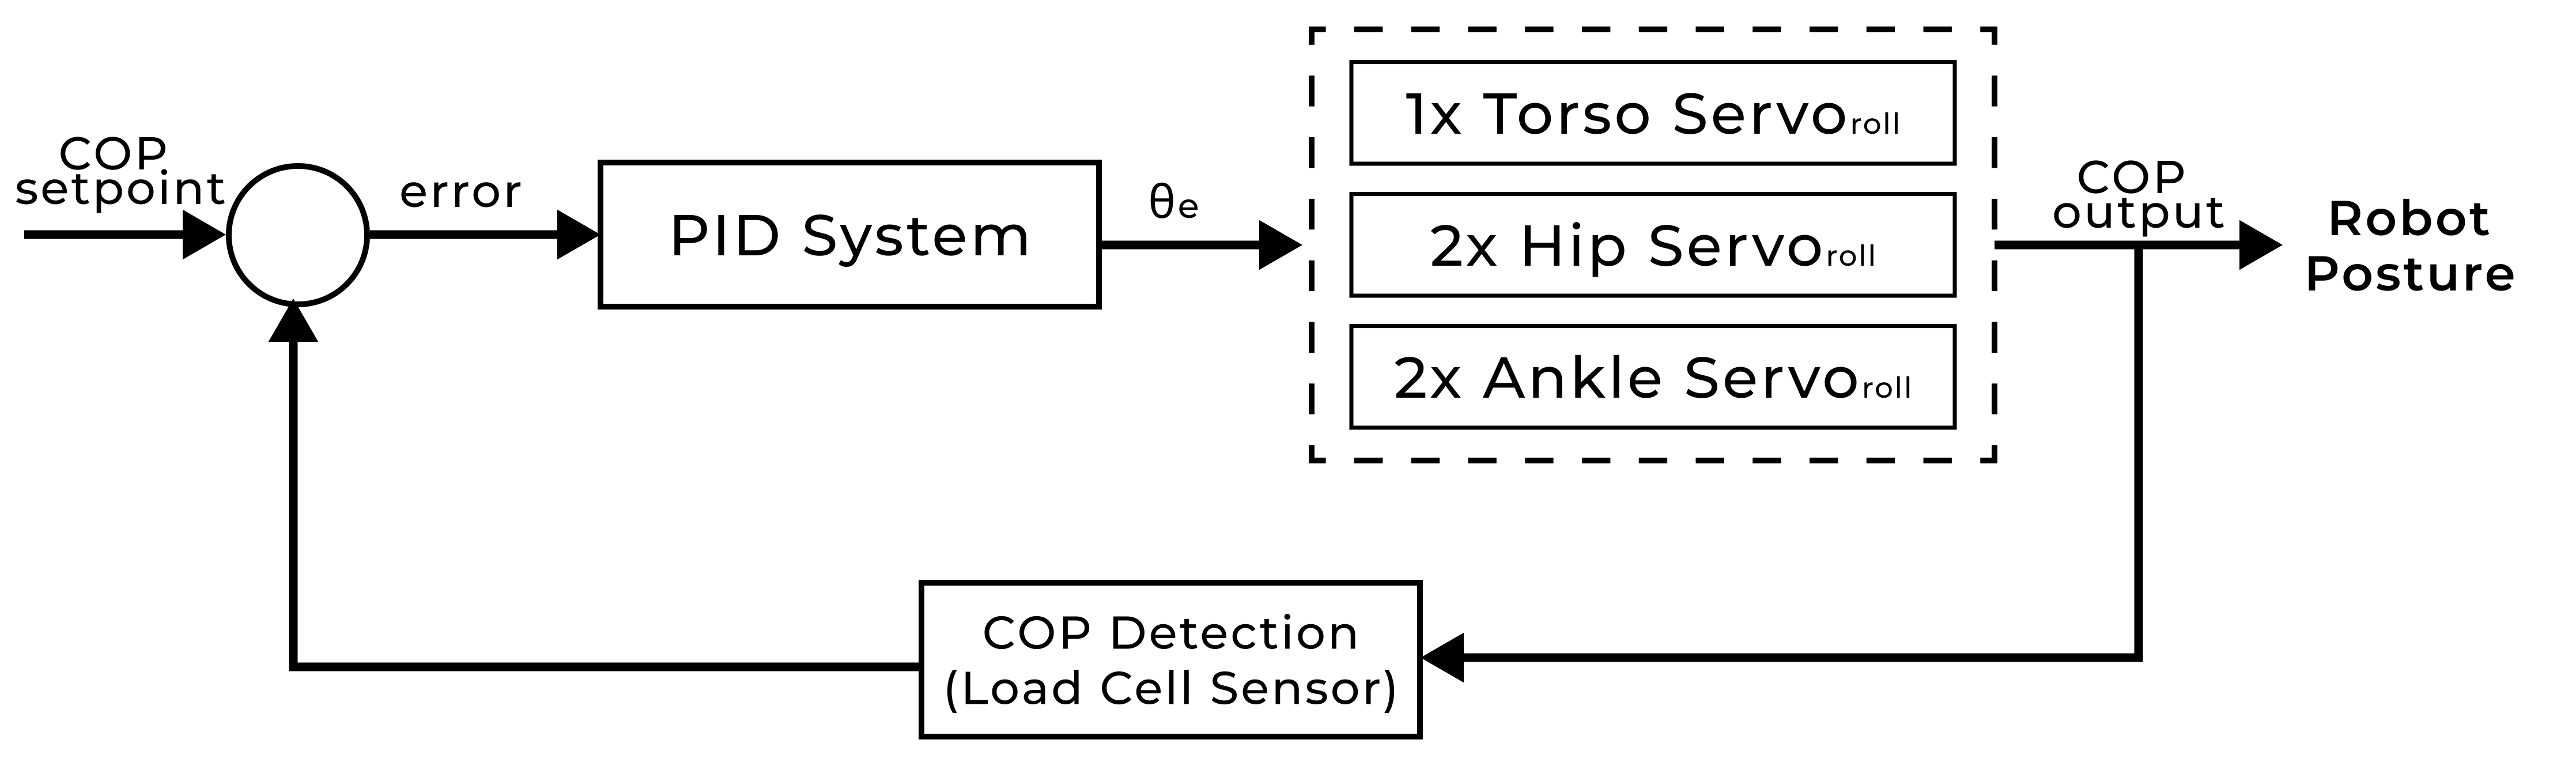
\includegraphics[width=0.4\textwidth]{gambar/pid_diagram.png}
      \caption{Diagram Sistem Kontrol PID}
      \label{fig:Control_System}
    \end{figure}

    \hspace*{1em}  Gambar \ref{fig:Control_System} menunjukkan diagram sistem kontrol yang terdiri dari tiga blok utama: blok PID, blok servo sebagai kompensasi, dan blok pusat tekanan. Blok {PID System} menghitung nilai koreksi dengan persamaan \ref{eq:Koreksi_PID}. Dimana nilai error diperoleh dari selisih antara $COP_{setpoint}$ dan $COP_{input}$. Nilai koreksi ini digunakan untuk mengatur posisi servo pada blok servo sebagai kompensasi dengan menggunakan 5 servo yang mengatur posisi roll robot. Blok pusat tekanan menghitung posisi pusat tekanan pada telapak kaki robot dan menyediakan data ini sebagai input pada kontrol PID.

    \item Pengaturan Servo sebagai Kompensasi
    \label{subsec:servosettings}

    \hspace*{1em} Pada penelitian ini, servo yang digunakan untuk menjaga keseimbangan adalah servo yang mengatur posisi \textit{roll} robot. Servo tersebut terletak pada \textit{torso}, \textit{hip}, dan \textit{ankle}. Servo pada \textit{torso}, \textit{hip}, dan \textit{ankle}. Dengan mengatur beberapa sudut servo, robot dapat melakukan penyesuaian yang diperlukan untuk mempertahankan keseimbangan saat bergerak atau berdiri di permukaan yang tidak rata. Terdapat lima servo yang digunakan yang terdiri dari satu servo pada \textit{torso} (ID 1), dua servo pada masing-masing \textit{hip} (ID 4 dan ID 5), dan dua servo pada masing-masing \textit{hip} (ID 13 dan ID 14). Pengaturan servo sebagai kompensasi dapat dilihat pada Gambar \ref{fig:Controlled_Servo}, ditunjukkan oleh servo yang diwarnai biru.

    \begin{figure} [h] \centering
      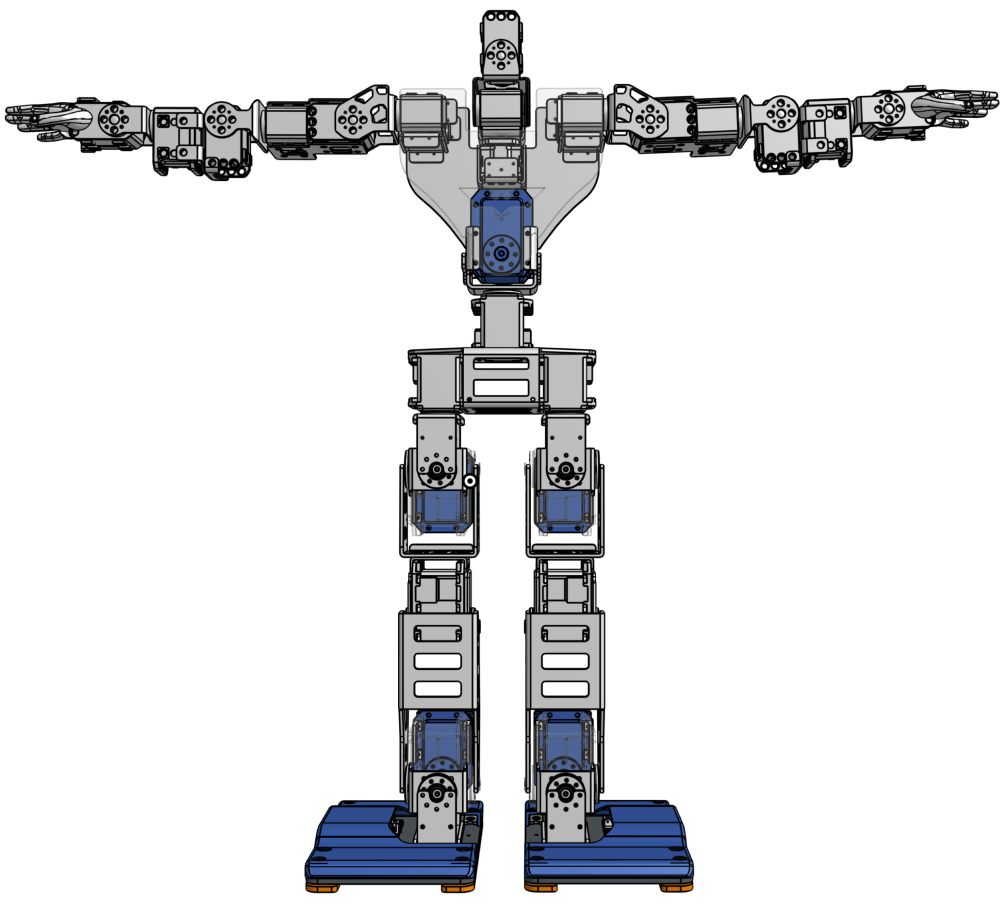
\includegraphics[width=0.4\textwidth]{gambar/controlled_servo.png}
      \caption{Pengaturan Servo sebagai Kompensasi Ditunjukkan dengan Warna Biru}
      \label{fig:Controlled_Servo}
    \end{figure}
    
    \begin{equation}
      \theta_{\mathrm{torso}} = \theta_{\mathrm{torso}} + (\mathrm{Koreksi}_{\mathrm{roll}} \cdot 0.8)
      \label{eq:Koreksi_Torso}
    \end{equation}
    
    \begin{equation}
      \theta_{\mathrm{hip}} = \theta_{\mathrm{hip}} + (\mathrm{Koreksi}_{\mathrm{roll}} \cdot 1)
      \label{eq:Koreksi_Hip}
    \end{equation}
    
    \begin{equation}
      \theta_{\mathrm{ankle}} = \theta_{\mathrm{ankle}} + (\mathrm{Koreksi}_{\mathrm{roll}} \cdot 0.4)
      \label{eq:Koreksi_Ankle}
    \end{equation}
    
    \hspace*{1em} Pada persamaan \ref{eq:Koreksi_Torso}, nilai koreksi digunakan untuk mengatur posisi servo pada \textit{torso} dengan faktor 0.8. Pada persamaan \ref{eq:Koreksi_Hip}, nilai koreksi digunakan untuk mengatur posisi servo pada \textit{hip} dengan faktor 1. Pada persamaan \ref{eq:Koreksi_Ankle}, nilai koreksi digunakan untuk mengatur posisi servo pada \textit{ankle} dengan faktor 0.4.  Pembagian skala nilai koreksi pada servo ditentukan dengan \textit{trial and error} dengan memperhatikan pengaruh pada setiap bagian tubuh robot dan spesiikasi dari servo yang digunakan.

    \hspace*{1em} 
\end{enumerate}
\section{Hasil dan Pembahasan}
\label{sec:hasildanpembahasan}

Dilakukan pengujian dan analisis terhadap perancangan dan implementasi yang telah di desain sebelumnya. Pengujian yang dilakukan meliputi pengujian Sensor Load Cell terhadap Robot dan Sistem Keseimbangan Robot. 

\begin{enumerate}[label=\Alph*.]

    \item Pengujian Karakterisasi Pada Masing-Masing Sensor Load Cell
    \label{subsec:hasil-pembahasan-karakterisasi}

        \hspace*{1em} Pengujian kalibrasi sensor load cell dilakukan dengan menggunakan lima bandul referensi massa (50g, 100g, 200g, 500g, dan 1000g). Bandul terkecil (50 gram) digunakan untuk menentukan koefisien gradien, sedangkan konstanta diperoleh dari \textit{tare weight} (titik 0 ketika \emph{load cell} tidak ada beban). Data hasil perhitungan ini kemudian digunakan untuk menghitung tingkat kesalahan (\textit{error}) dari setiap \emph{load cell} yang digunakan dengan membandingkan dengan massa aktual. 

        \begin{table}[h]
            \centering
            \caption{Hasil Karakterisasi Load Cell Pertama}
            \begin{tabular}{|c|c|c|}
                \hline
                \textbf{Berat Aktual (gr)} & \textbf{Load Cell 1 Pembacaan (gr)} & \textbf{Error (gr)} \\
                \hline
                50    & 50    & 0   \\
                100   & 101   & 1   \\
                200   & 202   & 2   \\
                500   & 505   & 5   \\
                1000  & 1004  & 4   \\
                \hline
            \end{tabular}
            \label{tab:Kalibrasi_Load_Cell_1}
        \end{table}

        \begin{table}[h]
            \centering
            \caption{Hasil Karakterisasi Load Cell Kedua}
            \begin{tabular}{|c|c|c|}
                \hline
                \textbf{Berat Aktual (gr)} & \textbf{Load Cell 2 Pembacaan (gr)} & \textbf{Error (gr)} \\
                \hline
                50        & 50        & 0   \\
                100       & 100       & 0   \\
                200       & 200       & 0   \\
                500       & 500       & 0   \\
                1000      & 994       & 6   \\           
                \hline
        \end{tabular}
        \label{tab:Kalibrasi_Load_Cell_2}
        \end{table}

        \begin{table}[h]
            \centering
            \caption{Hasil Karakterisasi Load Cell Ketiga}
            \begin{tabular}{|c|c|c|}
                \hline
                \textbf{Berat Aktual (gr)} & \textbf{Load Cell 3 Pembacaan (gr)} & \textbf{Error (gr)} \\
                \hline
                50        & 50        & 0    \\    
                100       & 103       & 3    \\    
                200       & 203       & 3    \\    
                500       & 494       & 6    \\    
                1000      & 981       & 19   \\               
                \hline
        \end{tabular}
        \label{tab:Kalibrasi_Load_Cell_3}
        \end{table}

        \begin{table}[h]
            \centering
            \caption{Hasil Karakterisasi Load Cell Keempat}
            \begin{tabular}{|c|c|c|}
                \hline
                \textbf{Berat Aktual (gr)} & \textbf{Load Cell 4 Pembacaan (gr)} & \textbf{Error (gr)} \\
                \hline
                50        & 50        & 0   \\     
                100       & 97        & 3   \\     
                200       & 204       & 4   \\     
                500       & 500       & 0   \\     
                1000      & 1003      & 3   \\                
                \hline
        \end{tabular}
        \label{tab:Kalibrasi_Load_Cell_4}
        \end{table}
    
        
        \hspace*{1em} Hasil pengujian karakterisasi pada masing-masing \emph{load cell} menunjukkan adanya kesalahan pengukuran yang bervariasi, berkisar antara 0 hingga 19 gram. Kesalahan ini tidak linear, menunjukkan bahwa kesalahan pengukuran tidak konstan pada setiap \emph{load cell}. Meskipun demikian, persamaan linear masih dapat digunakan untuk menghitung massa aktual dari pembacaan \emph{load cell} meskipun tidak sepenuhnya akurat.

    \item Pengujian Tekanan Pada Telapak Kaki
    \label{subsec:hasil-pembahasan-tekanan}

        \hspace*{1em} Pengujian ini dilakukan untuk mendapatkan data tekanan yang dihasilkan oleh kaki kanan dan kaki kiri ketika diberikan beban secara merata. Data tekanan yang dihasilkan oleh kaki kanan dan kaki kiri dapat dilihat pada Tabel \ref{tab:pengukuran_berat_kaki_kiri} dan Tabel \ref{tab:pengukuran_berat_kaki_kanan}.

        \begin{table}[h!]
            \centering
            \caption{Tabel Pembacaan Tekanan untuk Kaki Kiri}
            \begin{tabular}{|c|c|c|}
                \hline
                \textbf{Berat Aktual (gr)} & \textbf{Pembacaan (gr)} & \textbf{Error (gr)} \\
                \hline
                50    & 52    & 2   \\
                100   & 110   & 10  \\
                200   & 220   & 20  \\
                300   & 304   & 4   \\
                500   & 512   & 12  \\
                700   & 701   & 1   \\
                1000  & 1050  & 50  \\
                1300  & 1325  & 25  \\
                1500  & 1512  & 12  \\
                1800  & 1788  & 12  \\
                \hline
                \textbf{Rata-rata Error (gr)} & \multicolumn{2}{c|}{\textbf{14.8}} \\
                \hline
            \end{tabular}
            \label{tab:pengukuran_berat_kaki_kiri}
        \end{table}

        \begin{table}[h!]
            \centering
            \caption{Tabel Pembacaan Tekanan untuk Kaki Kanan}
            \begin{tabular}{|c|c|c|}
                \hline
                \textbf{Berat Aktual (gr)} & \textbf{Pembacaan (gr)} & \textbf{Error (gr)} \\
                \hline
                50    & 46    & 4    \\
                100   & 98    & 2    \\
                200   & 215   & 15   \\
                300   & 325   & 25   \\
                500   & 505   & 5    \\
                700   & 722   & 22   \\
                1000  & 1025  & 25   \\
                1300  & 1347  & 47   \\
                1500  & 1500  & 0    \\
                1800  & 1819  & 19   \\
                \hline
                \textbf{Rata-rata Error (gr)} & \multicolumn{2}{c|}{\textbf{16.4}} \\
                \hline
            \end{tabular}
            \label{tab:pengukuran_berat_kaki_kanan}
        \end{table}

        \begin{figure}[h]
            \centering
            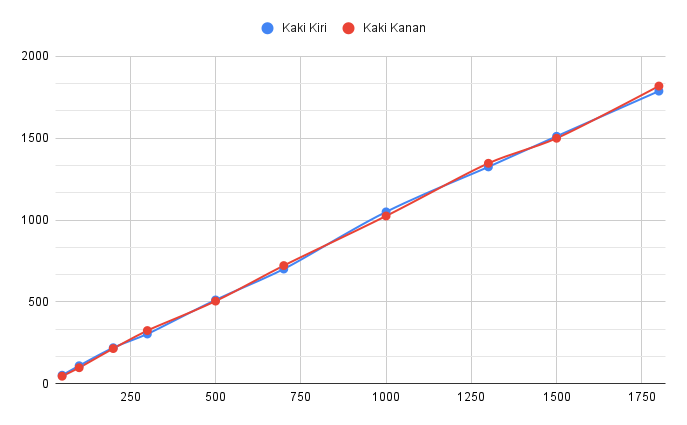
\includegraphics[width=0.4\textwidth]{gambar/chart_tekanan_kaki.png}
            \caption{Grafik Hubungan Antara Berat Aktual dan Pembacaan \emph{Load Cell} pada Kaki Kiri dan Kaki Kanan}
            \label{fig:tekanan_kaki}
        \end{figure}

        \hspace*{1em} Hasil pengukuran tekanan pada kaki kiri dan kaki kanan menunjukkan bahwa pembacaan \emph{load cell} pada kedua kaki memiliki kesalahan yang bervariasi, berkisar antara 0 hingga 50 gr. Kesalahan ini disebabkan oleh perbedaan karakteristik antara \emph{load cell} pada kaki kiri dan kaki kanan. Pada Gambar \ref{fig:tekanan_kaki} terlihat bahwa grafik tekanan yang dihasilkan oleh kaki kanan dan kaki kiri memiliki nilai pembacaan yang serupa.

    \item Pengujian Sistem Kontrol PID
    \label{subsec:hasil-pembahasan-pid}

        \hspace*{1em} Pengujian ini, dilakukan skenario pengujian ini meliputi analisis pengaruh masing-masing parameter PID. Hasil yang akan dianalisis adalah pengaruh parameter PID terhadap respon sistem dan hasil nilai \textit{Root Mean Square (RMS)} yang dihasilkan oleh sistem. Pengujian dilakukan dengan mengangkat kaki kanan atau kaki kiri dengan kemiringan 3 derajat. Berikut adalah hasil pengujian sistem keseimbangan robot.
        
        \begin{table}[h]
            \centering
            \caption{Hasil Pengujian Pengaruh Parameter P, Mengangkat Kaki Kiri Dengan Kemiringan 3 Derajat}
            \begin{tabular}{|c|c|c|c|c|}
                \hline
                \textbf{PID} & \textbf{Fall} & \textbf{Not Fall} & \textbf{Success} & RMS Error \\
                \hline
                $K_p = 0.00$ & 6 & 0 & 0   \% & 0.7598 \\
                $K_p = 0.05$ & 6 & 0 & 0   \% & 0.7690 \\
                $K_p = 0.10$ & 0 & 6 & 100 \% & 0.7779 \\
                $K_p = 0.15$ & 1 & 5 & 83  \% & 0.8145 \\
                $K_p = 0.20$ & 1 & 5 & 83  \% & 0.8870 \\
                $K_p = 0.25$ & 0 & 6 & 100 \% & 0.8801 \\            
                \hline
            \end{tabular}
            \label{tab:pengujian_p}
        \end{table}

        \hspace*{1em} Hasil pengujian pada Tabel \ref{tab:pengujian_p} menunjukkan bahwa nilai optimal parameter Kp untuk menjaga keseimbangan robot berkisar antara 0.10 hingga 0.20. Pada Kp = 0.00 dan Kp = 0.05, semua pengujian gagal dengan robot selalu jatuh. Nilai Kp = 0.10 menunjukkan performa terbaik dengan keberhasilan 100\% dalam menjaga keseimbangan pada gerakan mengangkat kaki kanan dan kiri di kemiringan 3 derajat. Nilai Kp yang lebih tinggi, seperti Kp = 0.25, menunjukkan penurunan performa. Hasil \textit{Root Mean Square} (RMS) menunjukkan error terkecil pada Kp = 0.10 dengan nilai 0.7779, menegaskan pentingnya pengaturan Kp yang tepat untuk stabilitas robot.

        \begin{table}[h]
            \centering
            \caption{Hasil Pengujian Pengaruh Parameter PI, Mengangkat Kaki Kanan Dengan Kemiringan 3 Derajat}
            \begin{tabular}{|c|c|c|c|c|}
                \hline
                \textbf{PID} & \textbf{Fall} & \textbf{Not Fall} & \textbf{Success} & RMS Error \\
                \hline
                $K_p = 0.1, K_i = 0.01$ & 2 & 4 & 66 \%  & 0.9701\\
                $K_p = 0.1, K_i = 0.02$ & 2 & 4 & 66 \%  & 0.8950\\
                $K_p = 0.1, K_i = 0.04$ & 1 & 5 & 83 \%  & 0.9345\\
                $K_p = 0.1, K_i = 0.10$ & 0 & 6 & 100 \% & 0.8471\\
                $K_p = 0.1, K_i = 0.20$ & 0 & 6 & 100 \% & 0.8980\\           
                \hline
            \end{tabular}
            \label{tab:pengujian_pi}
        \end{table}

        \hspace*{1em} Hasil pengujian pada Tabel \ref{tab:pengujian_pi} menunjukkan bahwa nilai optimal parameter Ki untuk menjaga keseimbangan robot berkisar antara 0.10 hingga 0.20. Pada Ki = 0.01 dan Ki = 0.02  robot gagal menjaga keseimbangan dengan tingkat keberhasilan 66\% hingga 83\%. Sebaliknya, pada Ki = 0.10 dan Ki = 0.20  robot berhasil menjaga keseimbangan dengan tingkat keberhasilan 100\% pada gerakan mengangkat kaki kanan dan kiri di kemiringan 3 derajat. Hasil \textit{Root Mean Square} (RMS) menunjukkan nilai terendah pada Ki = 0.10 sebesar 0.8471, sementara nilai tertinggi pada Ki = 0.01 sebesar 0.9701. Pengaruh Ki terhadap performa tidak terlalu signifikan, dan dalam beberapa kasus, nilai Ki yang lebih tinggi menurunkan performa sistem, menunjukkan bahwa parameter Ki dalam kontrol PID pada sistem ini tidak terlalu diperlukan.

        \begin{table}[h]
            \centering
            \caption{Hasil Pengujian Pengaruh Parameter PD, Mengangkat Kaki Kanan Dengan Kemiringan 3 Derajat}
            \begin{tabular}{|c|c|c|c|c|}
                \hline
                \textbf{PID} & \textbf{Fall} & \textbf{Not Fall} & \textbf{Success} & RMS Error \\
                \hline
                $K_p = 0.1, K_d = 0.005$ & 0 & 6 & 100 \% & 0.7143 \\
                $K_p = 0.1, K_d = 0.010$ & 0 & 6 & 100 \% & 0.7077 \\
                $K_p = 0.1, K_d = 0.020$ & 2 & 4 & 66  \% & 0.7262 \\
                $K_p = 0.1, K_d = 0.050$ & 5 & 1 & 16  \% & 0.7344 \\
                $K_p = 0.1, K_d = 0.100$ & 6 & 0 & 0   \% & 0.9231 \\          
                \hline
            \end{tabular}
            \label{tab:pengujian_pd}
        \end{table}

        \hspace*{1em} Hasil pengujian pada Tabel \ref{tab:pengujian_pd} menunjukkan bahwa nilai optimal parameter Kd untuk menjaga keseimbangan robot berkisar antara 0.005 hingga 0.020. Pada Kd = 0.005 dan Kd = 0.010, robot berhasil menjaga keseimbangan dengan tingkat keberhasilan 100\%. Namun, pada Kd = 0.020, tingkat keberhasilan menurun menjadi 66\%, dan pada Kd = 0.050, tingkat keberhasilan hanya 16\%. Pada Kd = 0.100, robot selalu jatuh. Hasil \textit{Root Mean Square} (RMS) menunjukkan nilai terendah pada Kd = 0.010 sebesar 0.7077, sementara nilai tertinggi pada Kd = 0.100 sebesar 0.9231. Pengaruh Kd terhadap performa sistem cukup signifikan, dan nilai Kd yang lebih tinggi menurunkan performa sistem.

\end{enumerate}
\section{Kesimpulan}
\label{sec:kesimpulan}

Pada Tugas Akhir ini, dilakukan pengembangan sistem keseimbangan berbasis load cell pada robot humanoid dengan 29 derajat kebebasan, khususnya pada robot tari humanoid VI-ROSE ITS. Sistem tertanam pada telapak kaki, yang menggunakan mikrokontroler ESP32-C3 untuk membaca sensor load cell, berhasil dibuat dengan kesalahan pengukuran berkisar antara 0-19 gram untuk setiap load cell, dan 0-50 gram untuk total telapak kaki. Rata-rata kesalahan tercatat sebesar 14.8 gram pada kaki kanan dan 14.6 gram pada kaki kiri. Robot berhasil menyeimbangkan diri ketika mengangkat kaki kanan atau kiri dengan menerapkan kontrol PID pada lima servo yang mengatur posisi roll robot, termasuk satu servo di torso, dua servo di hip, dan dua servo di ankle. Hasil manual tuning PID menunjukkan nilai $K_p=0.1$,dan $K_d =0.005$ yang memberikan performa terbaik dengan tingkat keberhasilan 100\% dalam menjaga keseimbangan robot. Pengujian dilakukan dengan gerakan mengangkat kaki kanan maupun kaki kiri dengan kemiringan 3 derajat.

Untuk pengembangan sistem ini di masa mendatang, disarankan untuk mengganti servo dengan model yang lebih kuat, seperti MX-64T, pada motor yang mengatur posisi roll robot. Selain itu, menggunakan data posisi pusat tekanan (CoP) untuk menentukan Zero Moment Point (ZMP) dapat membantu meningkatkan akurasi keseimbangan robot.
% Ucapan terima kasih jika ada
% \section{Ucapan Terima Kasih}
% \label{sec:ucapanterimakasih}

% Penulis mengucapkan terima kasih kepada Kementerian Riset, Teknologi, dan Pendidikan Tinggi Republik Indonesia atas \lipsum[1]

% Menambahkan semua entri dari pustaka tanpa perlu sitasi dalam teks
% \nocite{*}

% Menampilkan daftar pustaka dengan format IEEE
\bibliographystyle{IEEEtranN}
\bibliography{pustaka/pustaka.bib}

% Menyeimbangkan bagian akhir di kedua kolom
\balance

\end{document}
